%% =====================================================================
%% StoHyMoLAP -- Ramis basin manuscript (REVISED VERSION WITH CITATIONS)
%% Elsevier CAS single-column class (cas-sc.cls).
%%
%% REVISION NOTES:
%%  - Introduction, Methods, Discussion rewritten with targeted citations
%%    from the provided bibliography annotation package.
%%  - Citation style: \citep{} for parenthetical, \citet{} for narrative.
%%  - Placeholders marked %% [FILL] as before.
%% =====================================================================
\documentclass[a4paper,fleqn]{cas-sc}

\usepackage[authoryear,longnamesfirst]{natbib}
\usepackage{amsmath,amssymb}
\usepackage{booktabs}
\usepackage{graphicx}
\usepackage{tabularx}
\usepackage{threeparttable}
\usepackage{multirow}
\usepackage{siunitx}
\usepackage{xspace}
\usepackage{url}
\usepackage{float}
\usepackage{enumitem}

\begin{document}
\let\WriteBookmarks\relax
\def\floatpagepagefraction{1}
\def\textpagefraction{.001}

\shorttitle{Stochastic physical-ensemble quantiles for streamflow hybridization}
\shortauthors{Zevallos}

\title[mode = title]{Stochastic Physical-Ensemble Quantiles Improve Hybrid
Machine-Learning Simulation of Daily Streamflow in the High-Andean Ramis Basin}

% First author
\author[1]{Jose Zevallos}[orcid=0000-0002-6023-8665]
\cormark[1]
\ead{20240318@lamolina.edu.pe}
\credit{Conceptualization of this study, Methodology, Software, Writing -- original draft}

% Address/affiliation
\affiliation[1]{organization={Centro de Investigaci\'{o}n y Tecnolog\'{i}a del Agua (CITA), Universidad de Ingenier\'{i}a y Tecnolog\'{i}a (UTEC)},
                addressline={Jr. Medrano Silva 165, Barranco},
                city={Lima},
                postcode={15063},
                state={Lima},
                country={Peru}}

\cortext[1]{Corresponding author.}

%% =====================================================================
%% ABSTRACT
%% =====================================================================
\begin{abstract}
Hybrid hydrological modelling combines process-based structure with the
predictive flexibility of machine learning (ML), but often leaves unclear
which component drives improved streamflow prediction. We present
StoHyMoLAP, a reproducible and audit-controlled framework for daily
streamflow simulation in the high-Andean Ramis basin, within the Lake
Titicaca system of southern Peru. The framework couples a lumped RAMIS
rainfall--runoff core, an optional linear baseflow reservoir,
L\'{e}vy-type ($\alpha$-stable) stochastic perturbations, Monte Carlo
physical ensembles, and ML emulators trained from observed forcings or
from stochastic-ensemble descriptors. Nine experiments (E0--E8) were
evaluated over a common validation window from 8~January~2009 to
31~December~2020 ($n=4367$ daily samples), with temporal-leakage and
backend audits embedded in the evidence chain.

Quantile descriptors from the stochastic physical ensemble provided the
largest robust gain. The gradient-boosting quantile hybrid reached
NSE\,=\,0.740 and KGE\,=\,0.810, improving NSE by 0.311 relative to the
complete stochastic physical model and by 0.165 relative to the pure ML
baseline. Replacing ensemble-mean features with ensemble quantiles
alone added 0.114 NSE, showing that distributional physical descriptors
contain information not captured by a single mean trajectory. The
baseflow reservoir modestly improved the deterministic physical
baseline, whereas direct L\'{e}vy perturbations produced inconsistent
point-prediction gains. The stochastic physical bands were strongly
underdispersive (PICP\,=\,0.004 against a nominal 0.95 target), so the
ensemble is more useful as ML features than as calibrated predictive
uncertainty. The numerically best run (NSE\,=\,0.849, KGE\,=\,0.899,
RMSE\,=\,0.210~m$^3$\,s$^{-1}$) was labelled as GRU but executed as a
fallback multilayer perceptron on flattened sequences; it is not
evidence of recurrent-network superiority. These findings support
stochastic physical--ML hybridization while showing that uncertainty
calibration, low-flow correction and backend-aware reporting remain
essential for defensible hydrological modelling.
\end{abstract}

\begin{highlights}
\item Ensemble quantiles were the dominant driver of hybrid streamflow skill.
\item The quantile hybrid improved NSE by 0.311 over stochastic RAMIS.
\item L\'{e}vy perturbations informed ML features but underdispersed intervals.
\item Backend and leakage audits constrained claims for GRU-labelled runs.
\item The ablation separated memory, stochasticity, ML and descriptors.
\end{highlights}

\begin{keywords}
Daily streamflow simulation \sep Stochastic hydrological modelling \sep
Physical--machine learning hybridization \sep Ensemble quantiles \sep
Uncertainty diagnostics \sep High-Andean basin
\end{keywords}

\maketitle

%% =====================================================================
%% 1. INTRODUCTION
%% =====================================================================
\section{Introduction}\label{sec:introduction}

Reliable daily streamflow simulation remains a central problem in
surface-water hydrology, particularly in basins where observations are
sparse, hydroclimatic variability is strong and operational decisions
must still be supported by defensible discharge estimates
\citep{razavi2013streamflow,guo2021regionalization}. These conditions
are characteristic of many high-elevation Andean catchments. In the
Peruvian Altiplano, precipitation is strongly seasonal, monitoring
networks are sparse relative to the spatial heterogeneity of rainfall,
and discharge dynamics are shaped by the alternation between sharp
wet-season runoff response and sustained dry-season low flows
\citep{condom2004transient,zubieta2018hydrological,lima2025modeling}.
Such settings expose a persistent limitation of classical
rainfall--runoff modelling: even when a conceptual model captures the
main water-balance controls, simplified storage structures, uncertain
parameters and imperfect meteorological inputs can lead to structural
errors that become particularly visible under low-flow, flashy or
climatically contrasting conditions
\citep{van2013influence,nauditt2017conceptual,ragettli2014evaluation}.

Machine-learning (ML) models offer a complementary route because they
can learn nonlinear rainfall--runoff relations directly from data. Large
sample studies have shown that recurrent and other data-driven models
can match or outperform lumped conceptual models in daily streamflow
prediction, including in regional and basin-scale benchmarks
\citep{kratzert2019towards,lees2021benchmarking,arsenault2022continuous}.
However, predictive skill alone does not eliminate hydrological risk.
Purely data-driven models may be sensitive to distributional shifts,
training-period representativeness, extrapolation to extremes and the
absence of explicit physical constraints
\citep{frame2021deep,zhong2023developing}. In data-scarce basins, their
performance also depends strongly on whether antecedent hydrological
state information is available, because rainfall inputs alone may be
insufficient to represent catchment memory
\citep{adnan2021comparison,okkan2021embedding}. The practical question
is therefore not whether process-based or ML models are universally
superior, but how physical structure and empirical flexibility can be
combined without obscuring the source of any improvement.

Hybrid physical--ML modelling addresses this question by using process
simulations, physically derived states or synthetic physically
consistent samples as inputs to an empirical emulator. This strategy has
improved runoff simulation in several configurations, including
conceptual-model correction, nested hybrid rainfall--runoff modelling,
physics-guided deep learning and process-driven deep learning
\citep{mekonnen2015hybrid,mohammadi2022ihacres,okkan2021embedding,yang2020physical,xie2021physics,li2024process,zhu2025hybrid}.
Most of these studies, however, pass forward a deterministic physical
trajectory. That design preserves part of the process information but
collapses the conditional distribution of the simulated response into a
single value. For stochastic rainfall--runoff transformation, this is a
strong simplification: uncertainty in precipitation, model structure and
hydrological memory propagates nonlinearly into discharge and can alter
both peak timing and magnitude
\citep{gabellani2007propagation,hong2006uncertainty}. It also limits the
ability of the hybrid model to exploit distributional descriptors such
as ensemble quantiles, which are closely related to hydrological
signatures and to probabilistic forecasting diagnostics
\citep{guo2021regionalization,papacharalampous2022review}.

A recent stochastic hybridization study by
\citet{houenafa2025hybridization} showed that mean and quantile
descriptors of a L\'{e}vy-driven stochastic HyMoLAP discharge ensemble
can improve ML-based rainfall--runoff prediction. This result is
important because it moves physical--ML hybridization from deterministic
state correction toward distribution-aware physical descriptors. Yet it
also leaves three issues unresolved. First, the gain from the hybrid
pipeline may come from several components---hydrological memory,
stochastic perturbations, the ML correction itself or the use of
quantile rather than mean ensemble descriptors---and these effects are
not identifiable from a single best-model comparison. Second, a
stochastic ensemble that improves point prediction is not necessarily a
calibrated predictive interval; coverage, sharpness and interval scores
must be evaluated separately. Third, reproducibility claims require that
reported model labels match the backend that actually produced the
results, especially when deep-learning architectures have software
fallbacks or implementation contingencies.

This study addresses these gaps through StoHyMoLAP, an audited
stochastic physical--ML framework for daily streamflow simulation in the
high-Andean Ramis basin, the principal tributary of Lake Titicaca. The
framework couples a lumped RAMIS rainfall--runoff core, an optional
linear baseflow reservoir, L\'{e}vy-type stochastic perturbations,
Monte Carlo physical ensembles and ML emulators trained either from
observed forcings or from physical-ensemble descriptors. The purpose is
not to introduce another best-performing hybrid model, but to decompose
which components are responsible for performance gains. Nine controlled
experiments (E0--E8; Table~\ref{tab:experiment-matrix}) are therefore
evaluated over a common validation window using a single workflow
(Fig.~\ref{fig:method-workflow}). The ablation design isolates the
incremental roles of baseflow memory, stochastic forcing, ML correction
and descriptor choice.

The manuscript makes four specific contributions. First, it transfers
stochastic physical--ML quantile hybridization to a high-Andean,
strongly seasonal and data-scarce Altiplano basin, providing a contrast
to previous applications outside this hydroclimatic setting. Second, it
shows whether ensemble mean or ensemble quantiles carry the more useful
physical information for ML correction. Third, it evaluates the same
stochastic ensemble both as a source of predictive features and as a
candidate uncertainty band through PICP, PINAW and Winkler diagnostics.
Fourth, it embeds temporal-leakage and backend audits into the evidence
chain, following the broader call for transparent and reproducible
hydrological modelling \citep{hall2021hydrologist}. A key audit finding
is stated explicitly: the experiments labelled as GRU in the current
run were executed with a fallback multilayer perceptron on flattened
sequences, not with a true recurrent backend. They are therefore
interpreted as GRU-labelled sequential hybrids under fallback execution,
not as evidence of recurrent-network superiority
\citep{kratzert2018rainfall}.

%% =====================================================================
%% 2. MATERIALS AND METHODS
%% =====================================================================
\section{Materials and methods}\label{sec:methods}

\subsection{Study area}\label{subsec:study-area}

The Ramis River is the largest tributary of Lake Titicaca and the
lake's principal surface inflow, draining roughly one third of the
Titicaca catchment in the Puno region of the Peruvian Altiplano
\citep{roche1992,lavado2012}. The broader Titicaca system receives
approximately 53\% of its annual water budget from riverine inflow,
with evaporation accounting for 91\% of losses \citep{cross2001}.
Observed lake levels have fluctuated by approximately 6~m over the past
century, driven primarily by interannual variability in precipitation
rather than by snowmelt, irrigation withdrawals or ice melt
\citep{lima2025,cross2001}. Simple mass-balance models for the system
reproduce the observed seasonal asymmetry---peak levels in April,
minimum in December---with amplitudes close to 0.74~m
\citep{cross2001,condom2004}, providing a useful physical reference
for the catchment-scale discharge dynamics studied here.

The Ramis basin lies in a high-altitude (above $\sim$3\,800~m~a.s.l.),
semi-arid Andean environment with a strongly unimodal seasonal
precipitation regime: a wet season concentrated between December and
March (approximately 60\% of annual totals in three months) and a
pronounced dry season from roughly April to November
\citep{condom2004}. The Altiplano climate is characterized by
significant interannual variability \citep{lima2025}, and the
precipitation gradient from north to south is marked, ranging from
about 750~mm\,yr$^{-1}$ in the north to well below 200~mm\,yr$^{-1}$
in the south \citep{condom2004}. This seasonality produces a markedly
intermittent, ``flashy'' hydrological response, with low and sustained
dry-season baseflow punctuated by sharp wet-season peaks---a regime
known to challenge both deterministic conceptual models
\citep{van2013,nauditt2017} and purely data-driven models
\citep{lees2021}. Conceptual models calibrated for the region have
shown that the streamflow response is dominated by groundwater storage
fluxes rather than direct routing of snowmelt, underscoring the
importance of baseflow representation \citep{nauditt2017}. Daily
discharge is gauged at the Puente Ramis station (SENAMHI-Per\'{u}).

%% [FILL] Confirm and insert, from SENAMHI/ANA, the EXACT gauged drainage
%% area, station coordinates, record period, units, and any normalization
%% applied to the discharge series.
The gauged drainage area is approximately
\textbf{[FILL: XX\,XXX]}~km$^2$, the station is located at
\textbf{[FILL: lat, lon]}, and the daily series covers
\textbf{[FILL: record period]}.

\subsection{Study data and temporal protocol}\label{subsec:data-protocol}

The modelling unit is a daily hydro-meteorological series with
precipitation ($P_t$), minimum and maximum temperature
($T_{\min,t}$, $T_{\max,t}$), potential evapotranspiration ($PET_t$)
and observed streamflow ($Q^{obs}_t$). Effective precipitation is
\begin{equation}
P^{eff}_t = \max(P_t - PET_t,\;0).
\label{eq:peff}
\end{equation}
All models are trained and validated under a strict chronological
split: calibration from 8~September~1991 to 31~December~2008,
validation from 8~January~2009 to 31~December~2020. The final
comparison is restricted to the common validation intersection of all
experiments, comprising $n=4367$ daily samples. This common-window
design avoids the well-documented problem of giving physical models more
validation days than ML or sequential models \citep{lees2021}, and
ensures that all performance contrasts are computed on an identical
set of observations.

The temporal protocol embodies the leakage-control principles
recommended by \citet{arsenault2022} and \citet{chen2013}: predictors
are constructed with non-negative lags only, sequence samples are
generated within each temporal subset, scalers are fitted exclusively
on training data, and flow-regime thresholds are estimated from
training observations alone. The full audit is summarized in
Table~\ref{tab:reproducibility}. Partitioning meteorological inputs
and observational scalers by temporal subset is particularly important
when stochastic ensemble summaries---which aggregate distributional
properties of the simulated discharge---are used as ML features:
fitting their normalization on the full sample would constitute a
subtle form of the temporal leakage documented by
\citet{arsenault2022}.

\subsection{Physical rainfall--runoff core}\label{subsec:physical-core}

Despite the term ``hydrodynamic'' sometimes appearing in the
user-facing workflow, the current StoHyMoLAP implementation is a lumped
stochastic rainfall--runoff simulator rather than a spatial
two-dimensional solver. The physical core is therefore described here
as a discharge-dynamics model. Its fast-flow component follows a
RAMIS-type state recurrence:
\begin{equation}
x_t = \left(1 - \frac{\mu}{\lambda}\right)x_{t-1} + P^{eff}_t,
\label{eq:ramis-state}
\end{equation}
where $\mu>0$ and $\lambda>0$ control memory and recession stability.
The constraint $0<\mu/\lambda<1$ prevents unstable or sign-changing
memory factors. The fast discharge trajectory $Q^{fast}_t$ is
\begin{equation}
Q^{fast}_t = Q^{fast}_{t-1}
  - \frac{\mu}{\lambda}\,Q_0
    \left(\frac{\max(Q^{fast}_{t-1},0)}{Q_0}\right)^{2\mu-1}
  + \frac{\alpha_A}{\lambda}\,x_{t-1}
  + \sigma\,Q^{fast}_{t-1}\,\Delta L_t,
\label{eq:ramis-fast}
\end{equation}
where $Q_0$ is the reference discharge, $\alpha_A$ is an empirical
conversion factor, $\sigma$ controls stochastic amplitude, and
$\Delta L_t$ is a L\'{e}vy-stable increment.
Negative simulated discharge is clipped to zero when the experiment
activates non-negative physical post-processing.

In line with \citet{harman2009}, the recurrence in Eqs.\
\ref{eq:ramis-state}--\ref{eq:ramis-fast} treats catchment-scale
nonlinearity as emerging from the aggregation of heterogeneous
storage elements rather than from local hydraulic nonlinearity. This
allows the parameter $\mu$ to be interpreted as a shape parameter
that implicitly encodes the heterogeneity of the storage ensemble,
consistent with the recession analysis framework of that work.

\subsection{Baseflow reservoir as hydrological memory}
\label{subsec:baseflow}

Hydrological memory is represented by an optional linear baseflow
reservoir. The theoretical basis for this component rests on the
observation that in semi-arid Andean catchments like the Ramis,
``the streamflow response is mostly consistent with flux from
groundwater storage'' \citep{nauditt2017}, and that models ignoring
this dynamics tend to overestimate seasonal low-flow periods and
underestimate high-flow periods \citep{nauditt2017}. Furthermore,
\citet{adnan2021comparison} demonstrated quantitatively that
including previous runoff (a proxy for storage memory) as a model
input ``considerably improves the accuracy [with] increments in RMSE
and MAE generally more than 90\%,'' and that ``excluding previous
runoff information from the model inputs or including only rainfall
information produces inaccurate models.''

Recharge to the store is proportional to effective precipitation:
\begin{equation}
R_t = c_r\,\alpha_A\,P^{eff}_t,
\label{eq:recharge}
\end{equation}
where $c_r\in[0,1]$ is a recharge coefficient. Storage and baseflow
discharge evolve as
\begin{align}
S_{b,t+1} &= \max\!\left(0,\;S_{b,t} + R_t - k_b S_{b,t}\right),
\label{eq:storage}\\
Q^{base}_t &= k_b\,S_{b,t},
\label{eq:qbase}
\end{align}
with $k_b\in[0.001,0.5]$, and the total physical discharge is
\begin{equation}
Q^{phys}_t = \max\!\left(Q^{fast}_t + Q^{base}_t,\;0\right).
\label{eq:qtotal}
\end{equation}
This component is activated in E1, E3 and the hybrid configurations.
Its isolated effect is quantified through the E1--E0 and E3--E2
ablation contrasts in Table~\ref{tab:ablation}.

\subsection{L\'{e}vy stochastic perturbations and Monte Carlo ensemble}
\label{subsec:levy}

The stochastic physical experiments inject $\alpha$-stable L\'{e}vy
increments into Eq.~\ref{eq:ramis-fast}. Random variates are
generated with the Chambers--Mallows--Stuck method
\citep{chambers1976cms}, parameterized by stability $\alpha$,
skewness $\beta$, location and scale. The use of heavy-tailed
$\alpha$-stable perturbations rather than Gaussian noise is motivated
by the documented importance of higher moments in hydrological
ensemble prediction: \citet{abaza2017} noted that ``biases occur not
only in relation to the mean, but also in higher statistical moments
of the predictive distribution,'' and \citet{atger1999} showed
empirically that ``poorer sampling of the higher moments of the
distribution'' limits skill when ensemble members are insufficient to
characterize the tail. In the strongly seasonal, intermittent Ramis
regime, where the distribution of daily discharge is far from
Gaussian, heavy-tailed perturbations provide a more conservative and
physically plausible stochastic forcing than Gaussian equivalents.

For each calibrated parameter set, a Monte Carlo ensemble of $N$
trajectories is simulated, following the two-step design---stochastic
input generation followed by hydrological simulation---recommended by
\citet{gabellani2007} and \citet{hong2006}. The ensemble is
summarized at each time step by the mean, median, standard deviation
and quantiles
\begin{equation}
\{q_{0.01},\;q_{0.05},\;q_{0.25},\;q_{0.50},\;q_{0.75},
  \;q_{0.95},\;q_{0.99}\},
\label{eq:quantiles}
\end{equation}
as well as interquantile widths such as $q_{0.95}-q_{0.05}$ and
$q_{0.75}-q_{0.25}$. The use of quantile-based representations is
motivated by their robustness to fat-tailed distributions and outliers
\citep{swiderski2016}, which makes them suitable summaries of an
$\alpha$-stable ensemble even when the distribution cannot be
characterized by its first two moments alone. These descriptors serve
two purposes: direct stochastic physical simulation in E2 and E3,
and physically informed features for hybrid emulators in E5--E8. The
uncertainty diagnostics derived from these ensembles are reported in
Table~\ref{tab:uncertainty} and Fig.~\ref{fig:uncertainty-diagnostics}.

\subsection{Machine-learning emulator architecture}
\label{subsec:emulator}

The ML component is a supervised emulator mapping feature vectors
$\mathbf{z}_t$ to simulated discharge:
\begin{equation}
\hat{Q}_t = f_\theta(\mathbf{z}_t),
\label{eq:emulator}
\end{equation}
followed by non-negative clipping:
\begin{equation}
Q^{sim}_t = \max(\hat{Q}_t,\;0).
\label{eq:ml-clipping}
\end{equation}

Three feature families are used. First, the pure ML baseline (E4) uses
observed forcing variables and their non-negative lags. The inclusion
of lagged observed discharge as a feature is consistent with the
strong empirical evidence that lagged runoff markedly improves ML-based
rainfall--runoff models, and that pure meteorological inputs alone are
``inappropriate for hourly runoff prediction''
\citep{adnan2021comparison}. Second, mean-based hybrids (E5, E7) use
the ensemble mean of the stochastic physical simulation, arranged as
temporal sequences for the sequential emulator. Third, quantile-based
hybrids (E6, E8) use ensemble quantiles and spread descriptors,
preserving information about the shape and tail behaviour of the
physical ensemble. The theoretical justification for the move from
mean to quantile descriptors rests on the argument of
\citet{papacharalampous2022} that ``there are two ways for improving
predictive performance: (i) improving the prediction algorithm; and
(ii) discovering new informative predictors,'' and that quantile
representations of ensemble distributions constitute precisely the
kind of additional informative predictor that enables probabilistic
post-processing to go beyond first-moment correction.

The tabular emulator is labelled as XGB. If the \texttt{xgboost}
package is available, the implementation uses
\texttt{XGBRegressor}~\citep{chen2016xgboost}; otherwise it falls
back to \texttt{HistGradientBoostingRegressor}
\citep{friedman2001gbm}. In the current evidence package, the
XGB-labelled models used the \texttt{sklearn\_hgb} backend
(Table~\ref{tab:backend}); both are gradient-boosted tree ensembles,
so the XGB-labelled results remain valid evidence of gradient-boosting
hybridization. Hyperparameter search uses randomized search with
\texttt{TimeSeriesSplit}, preserving temporal ordering during model
selection \citep{chen2013}.

The sequential emulator is labelled as GRU \citep{cho2014gru} and can
use TensorFlow/Keras or PyTorch GRU layers when available. If neither
backend is installed, the implementation flattens each sequence and
trains an \texttt{MLPRegressor}. The current E7 and E8 runs used this
fallback. Therefore, in all Results and Discussion statements, E7 and
E8 are interpreted as GRU-labelled sequential hybrids with fallback
MLP backends, not as true recurrent GRU models.

\subsection{Calibration objective}\label{subsec:calibration}

The physical and stochastic models are calibrated with a scalar
multi-objective score combining efficiency, distributional agreement,
bias and interval coverage:
\begin{equation}
J = \frac{w_{NSE}(1-NSE) + w_{KGE}(1-KGE)
  + w_{PBIAS}\left|\frac{PBIAS}{100}\right|
  + w_{cov}|c^*-PICP|}{w_{active}},
\label{eq:objective}
\end{equation}
where $c^*=0.95$ is the target coverage and $w_{active}$ is the sum
of active weights. The default weights are $w_{NSE}=0.40$,
$w_{KGE}=0.30$, $w_{PBIAS}=0.15$ and $w_{cov}=0.15$. When a model
provides no prediction intervals, the coverage term is omitted and
remaining weights are renormalized.

This composite criterion follows the recommendation of
\citet{pushpalatha2012} that ``there is no single criterion that can
evaluate model performance in all cases,'' and the argument of
\citet{papacharalampous2022} that ``scoring rules that evaluate either
reliability or sharpness alone are not proper for the task.'' The
inclusion of KGE as a complementary metric to NSE is motivated by its
well-known decomposition into correlation, variability and bias
components \citep{gupta2009kge}, which makes it less sensitive than NSE
to the systematic underweighting of low-flow errors discussed by
\citet{pushpalatha2012}. The coverage term penalizes underdispersive
stochastic bands \citep{franz2011,abaza2017}.

\subsection{Experimental matrix and ablation design}
\label{subsec:matrix}

The experimental matrix in Table~\ref{tab:experiment-matrix} isolates
the contribution of each modelling component. E0 and E1 test
deterministic RAMIS without and with baseflow. E2 and E3 test L\'{e}vy
stochasticity without and with baseflow. E4 is a pure ML baseline.
E5 and E6 are XGB-labelled hybrids using mean and quantile
physical-ensemble features, respectively. E7 and E8 extend these to
sequential emulators with the fallback MLP backend in the current run.

\begin{table*}[t]
\caption{Controlled experimental matrix. Backend entries report the
actual backend used in the current run.}
\label{tab:experiment-matrix}
\centering
\small
\begin{tabular*}{\textwidth}{@{\extracolsep{\fill}}lllllll@{}}
\toprule
Experiment & Family & L\'{e}vy & Baseflow & Emulator & Features
  & Backend used \\
\midrule
E0\_RAMIS\_DET\_NOBF   & physical RAMIS & no  & no  & none
  & physical\_only & physical \\
E1\_RAMIS\_DET\_BF     & physical RAMIS & no  & yes & none
  & physical\_only & physical \\
E2\_RAMIS\_LEVY\_NOBF  & RAMIS-L\'{e}vy & yes & no  & none
  & physical\_only & physical \\
E3\_RAMIS\_LEVY\_BF    & RAMIS-L\'{e}vy & yes & yes & none
  & physical\_only & physical \\
E4\_ML\_PURE\_XGB      & pure ML        & no  & no  & XGB-labelled
  & observed\_forcing & sklearn\_hgb \\
E5\_HYB\_XGB\_MEAN     & hybrid         & yes & yes & XGB-labelled
  & ensemble mean & sklearn\_hgb \\
E6\_HYB\_XGB\_QUANTILES & hybrid        & yes & yes & XGB-labelled
  & ensemble quantiles & sklearn\_hgb \\
E7\_HYB\_GRU\_MEAN     & sequential hybrid & yes & yes & GRU-labelled
  & mean sequence & fallback MLP \\
E8\_HYB\_GRU\_QUANTILES & sequential hybrid & yes & yes & GRU-labelled
  & quantile sequence & fallback MLP \\
\bottomrule
\end{tabular*}
\end{table*}

\subsection{Relation to prior stochastic physical--ML hybridization}
\label{subsec:relation}

The idea of feeding statistical descriptors of a stochastic physical
ensemble to an ML emulator follows \citet{houenafa2025}. The present
study is complementary rather than overlapping. \citet{houenafa2025}
\emph{demonstrate} that stochastic descriptor hybridization improves
point prediction in a single basin and report a best hybrid model. The
present study instead \emph{decomposes} the same family of pipelines:
(i)~it isolates the marginal contribution of hydrological memory,
stochastic noise, ML correction and descriptor choice through nine
controlled ablation contrasts on a common validation window; (ii)~it
adds a linear baseflow reservoir as an explicit memory component and
evaluates it in isolation; (iii)~it reports KGE and PBIAS alongside
NSE/RMSE and adds flow-regime error analysis; (iv)~it evaluates the
stochastic bands as \emph{calibrated} uncertainty using coverage
diagnostics (PICP, PINAW, Winkler) following the probabilistic
verification framework of \citet{franz2011} and \citet{abaza2017};
and (v)~it embeds a leakage-and-backend audit, including the
disclosure that the GRU-labelled runs used a fallback MLP
\citep{hall2021}. The application setting also differs markedly: a
high-Andean, strongly seasonal Altiplano basin versus a West-African
basin.

\subsection{Evaluation metrics and audits}\label{subsec:evaluation}

Model performance is evaluated with NSE \citep{nash1970nse}, KGE
\citep{gupta2009kge}, RMSE, MAE, PBIAS and $R^2$.
Performance is interpreted following \citet{moriasi2015}. Regime
metrics are computed for low, mid and high flows using thresholds
estimated from calibration observations only; NSE is interpreted
with caution for low flows, where observed variance is small
\citep{pushpalatha2012}. Stochastic reference bands are evaluated
with PICP, PINAW, mean prediction interval width (MPIW) and Winkler
score \citep{franz2011,papacharalampous2022}. An ensemble is
considered well-calibrated when PICP approaches the nominal level
and PINAW is minimized subject to that coverage constraint
\citep{atger1999,abaza2017}. The final audit checks temporal split
integrity, feature construction, target leakage, backend metadata,
common-window consistency and non-negative ML post-processing
(Table~\ref{tab:reproducibility}).

\begin{figure*}[t]
\centering
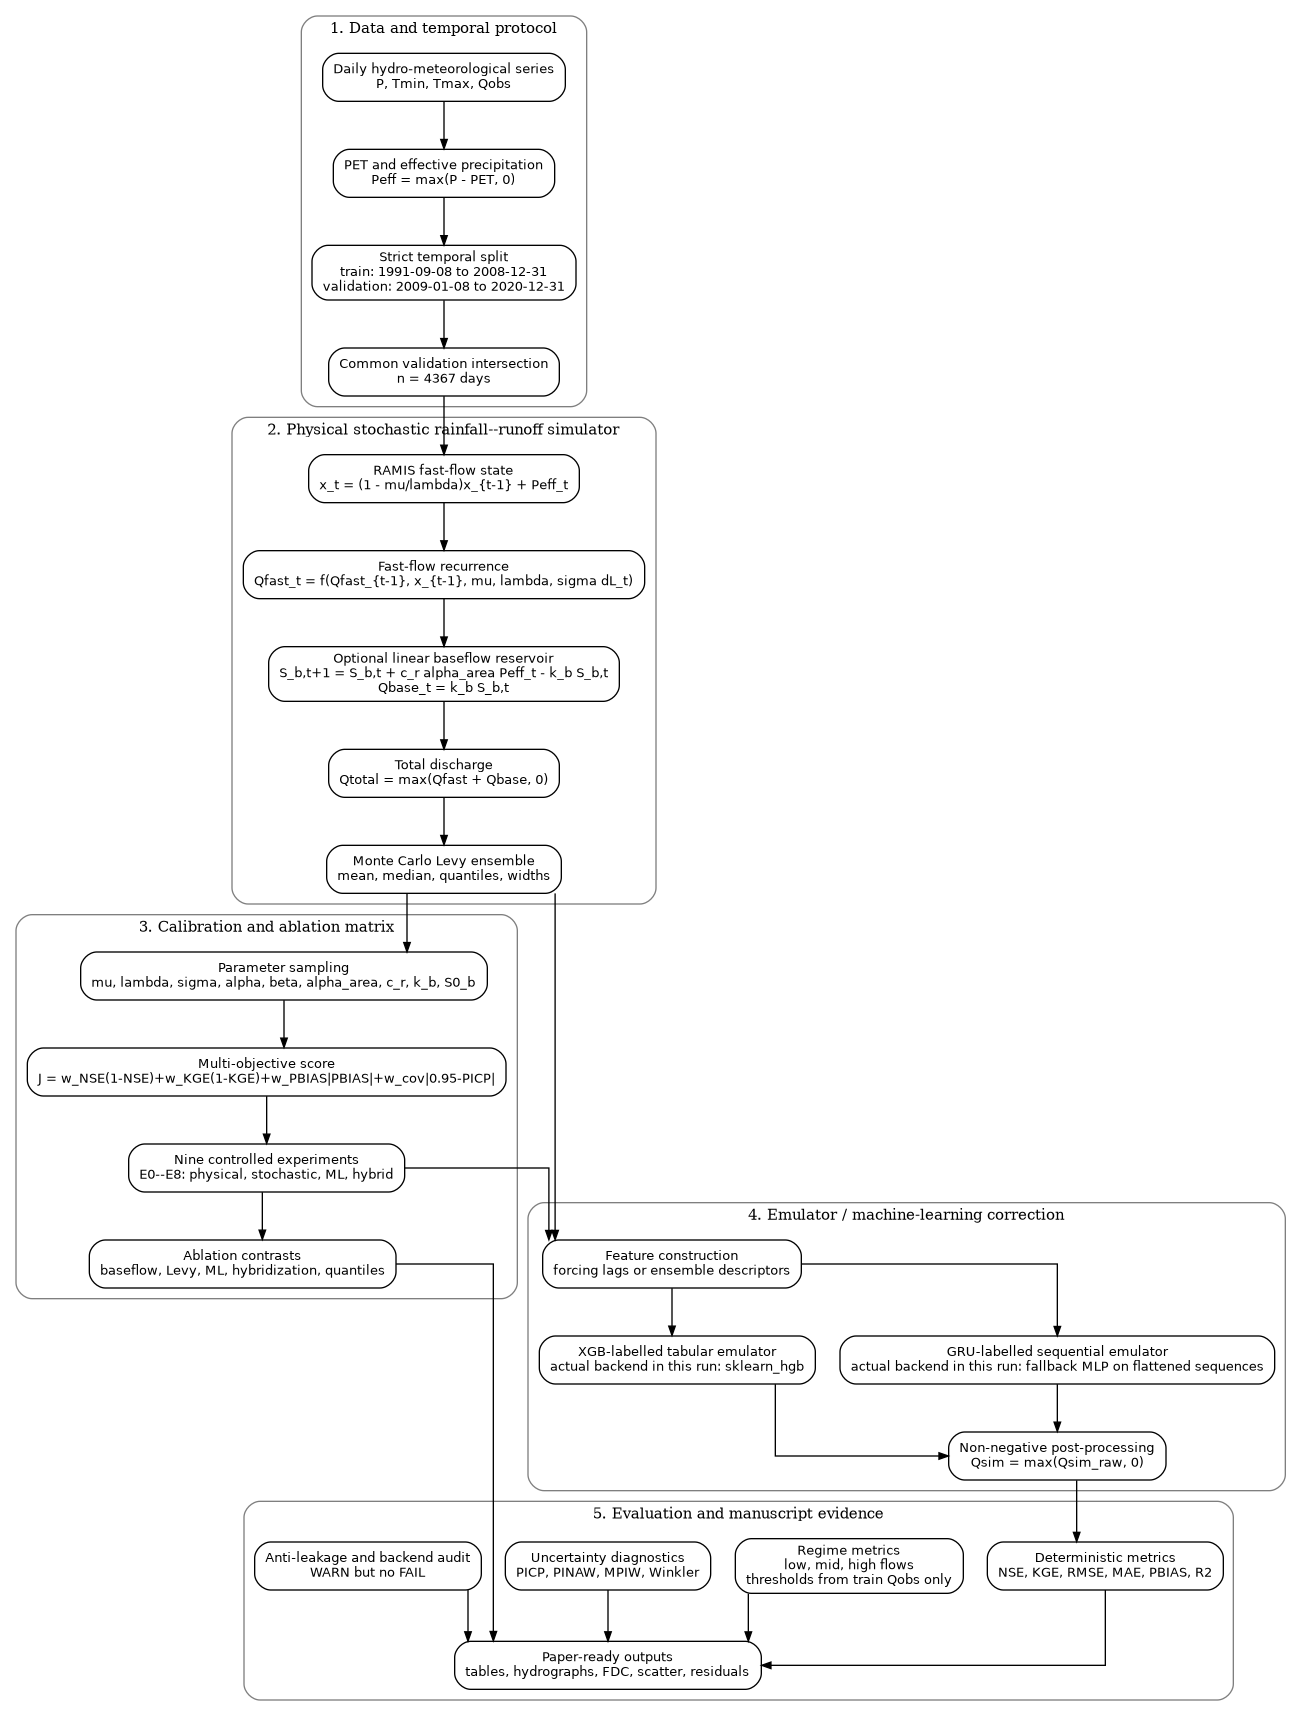
\includegraphics[width=0.96\textwidth]{figures/method_workflow.png}
\caption{Hierarchical workflow of the StoHyMoLAP methodology, from
daily hydro-meteorological data to physical simulation, stochastic
ensemble generation, emulator training, ablation comparison and
audit-controlled manuscript evidence.}
\label{fig:method-workflow}
\end{figure*}

%% =====================================================================
%% 3. RESULTS
%% =====================================================================
\section{Results}\label{sec:results}

\subsection{Common-window ranking}\label{subsec:ranking-results}

All experiments were evaluated over the common validation window
described in Section~\ref{subsec:data-protocol}.
Table~\ref{tab:ranking} and Fig.~\ref{fig:metric-ranking} summarize
the final ranking. The strongest \emph{robust} configuration was
E6\_HYB\_XGB\_QUANTILES, with NSE\,=\,0.740 and KGE\,=\,0.810: it is
the best model whose reported architecture matches the backend that
actually ran, and it provides the most defensible evidence for
quantile-based physical--ML hybridization. The top-ranked
configuration overall was E8\_HYB\_GRU\_QUANTILES, with
NSE\,=\,0.849, KGE\,=\,0.899, RMSE\,=\,0.210~m$^3$\,s$^{-1}$,
MAE\,=\,0.124~m$^3$\,s$^{-1}$ and PBIAS\,=\,1.579\%; however, this
result must be read under the backend caveat in Table~\ref{tab:backend}
because E8 was executed as a fallback MLP on flattened sequences.
All four hybrid models outperformed the pure ML baseline (E4,
NSE\,=\,0.575), which in turn outperformed all physical baselines
in NSE and RMSE, consistent with the pattern reported by
\citet{arsenault2022} and \citet{lees2021benchmarking} for LSTM-based
models in ungauged catchments.

\begin{table*}[t]
\caption{Final common-window ranking. Metrics are computed on 4367
validation samples from 8 January 2009 to 31 December 2020.}
\label{tab:ranking}
\centering
\small
\begin{tabular*}{\textwidth}{@{\extracolsep{\fill}}rlllllll@{}}
\toprule
Rank & Experiment & NSE & KGE & RMSE & MAE & PBIAS & Backend \\
\midrule
1 & E8\_HYB\_GRU\_QUANTILES   & 0.849 & 0.899 & 0.210 & 0.124
  & 1.579 & fallback\_mlp\_on\_flattened\_sequences \\
2 & E6\_HYB\_XGB\_QUANTILES   & 0.740 & 0.810 & 0.275 & 0.162
  & 0.927 & sklearn\_hgb \\
3 & E7\_HYB\_GRU\_MEAN        & 0.686 & 0.789 & 0.302 & 0.192
  & 1.644 & fallback\_mlp\_on\_flattened\_sequences \\
4 & E5\_HYB\_XGB\_MEAN        & 0.626 & 0.715 & 0.330 & 0.210
  & 2.007 & sklearn\_hgb \\
5 & E4\_ML\_PURE\_XGB         & 0.575 & 0.661 & 0.352 & 0.223
  & 0.742 & sklearn\_hgb \\
6 & E1\_RAMIS\_DET\_BF        & 0.438 & 0.714 & 0.405 & 0.248
  & 0.860 & physical \\
7 & E3\_RAMIS\_LEVY\_BF       & 0.429 & 0.725 & 0.408 & 0.255
  & -1.218 & physical \\
8 & E2\_RAMIS\_LEVY\_NOBF     & 0.427 & 0.717 & 0.409 & 0.268
  & -7.551 & physical \\
9 & E0\_RAMIS\_DET\_NOBF      & 0.414 & 0.713 & 0.413 & 0.270
  & -5.865 & physical \\
\bottomrule
\end{tabular*}
\end{table*}

\begin{figure}[t]
\centering
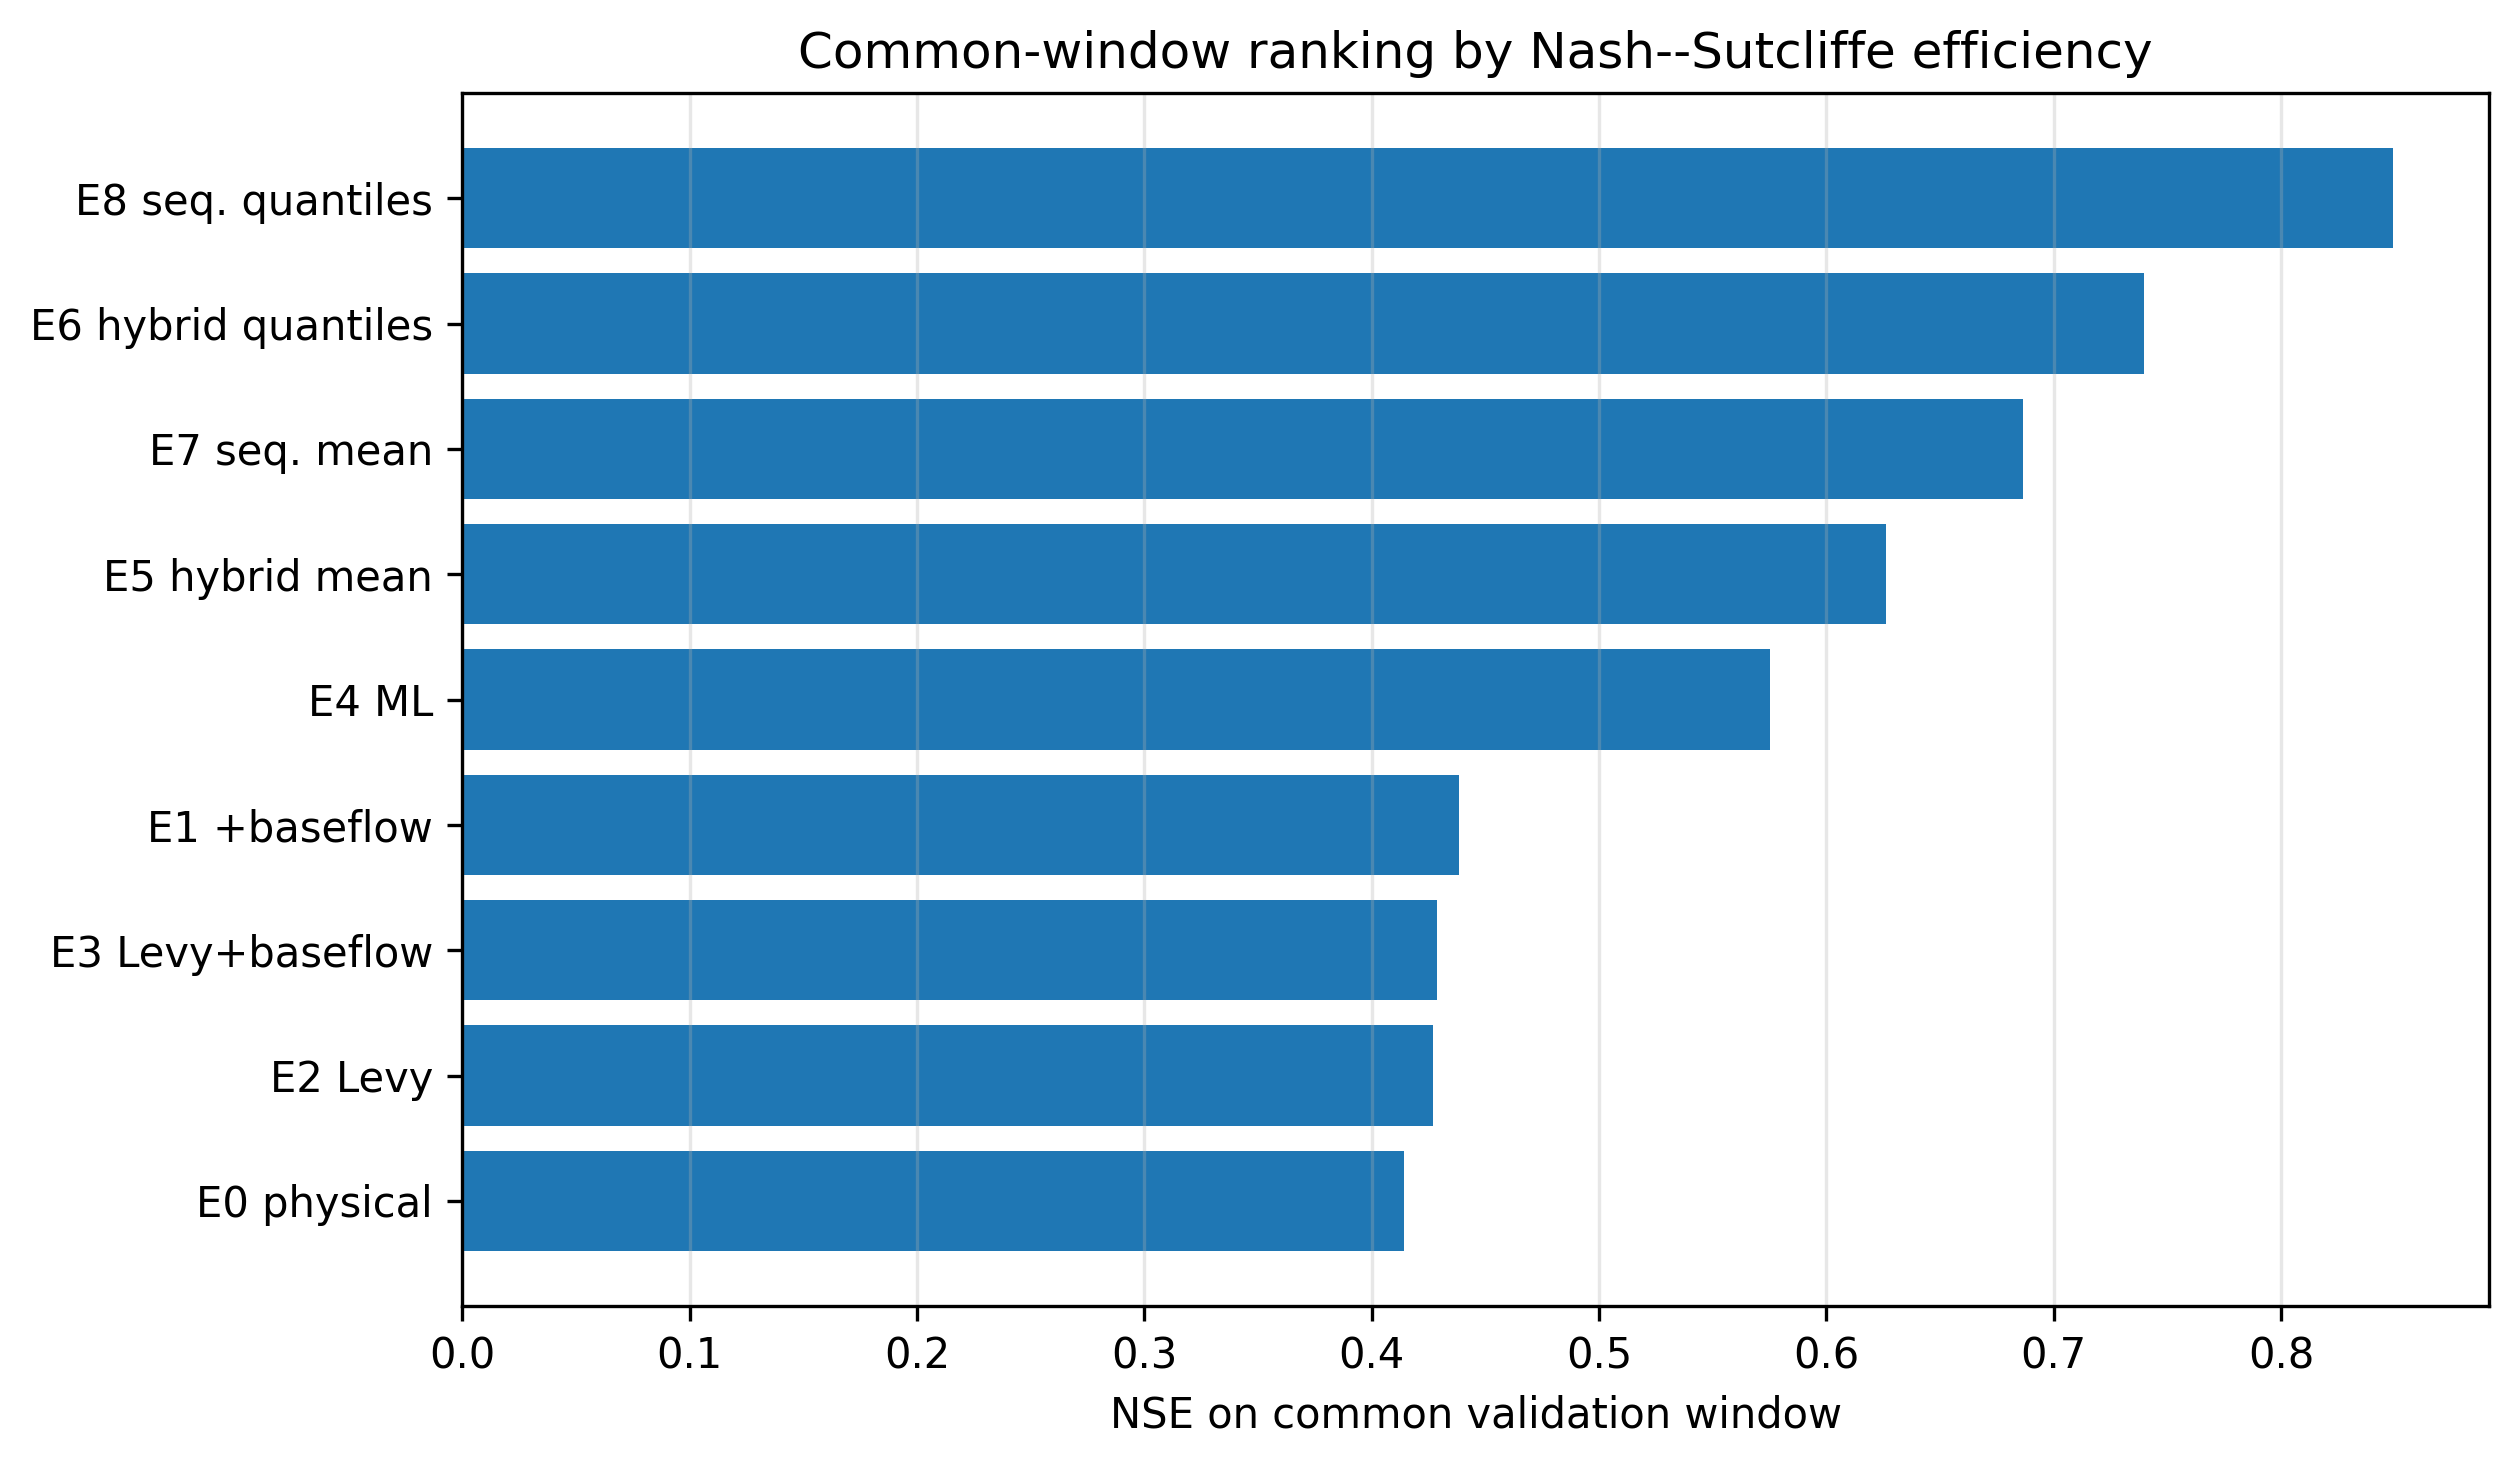
\includegraphics[width=0.95\linewidth]{figures/metric_ranking_nse.png}
\caption{Ranking of all experiments by common-window NSE. Numerical
values correspond to Table~\ref{tab:ranking}.}
\label{fig:metric-ranking}
\end{figure}

\subsection{Hydrograph and flow-duration behaviour}
\label{subsec:hydro-results}

The validation hydrograph in Fig.~\ref{fig:hydrograph-common}
compares observed and simulated daily discharge for the representative
models. Hybrid models better track temporal variability than the
physical-only baselines, while the flow-duration curves in
Fig.~\ref{fig:fdc-common} show that quantile-based hybridization
improves distributional agreement across a broad range of exceedance
probabilities. These visual diagnostics are consistent with the
metric improvements in Table~\ref{tab:ranking}, but they also reveal
persistent discrepancies during low-flow periods. The pronounced
collapse of the E0 physical model in the high-exceedance tail of the
FDC is particularly informative: it reflects the inability of a
single-reservoir deterministic model to maintain positive discharge
during dry-season recession, a limitation documented for similar
semi-arid Andean settings by \citet{nauditt2017} and \citet{van2013}.

\begin{figure*}[t]
\centering
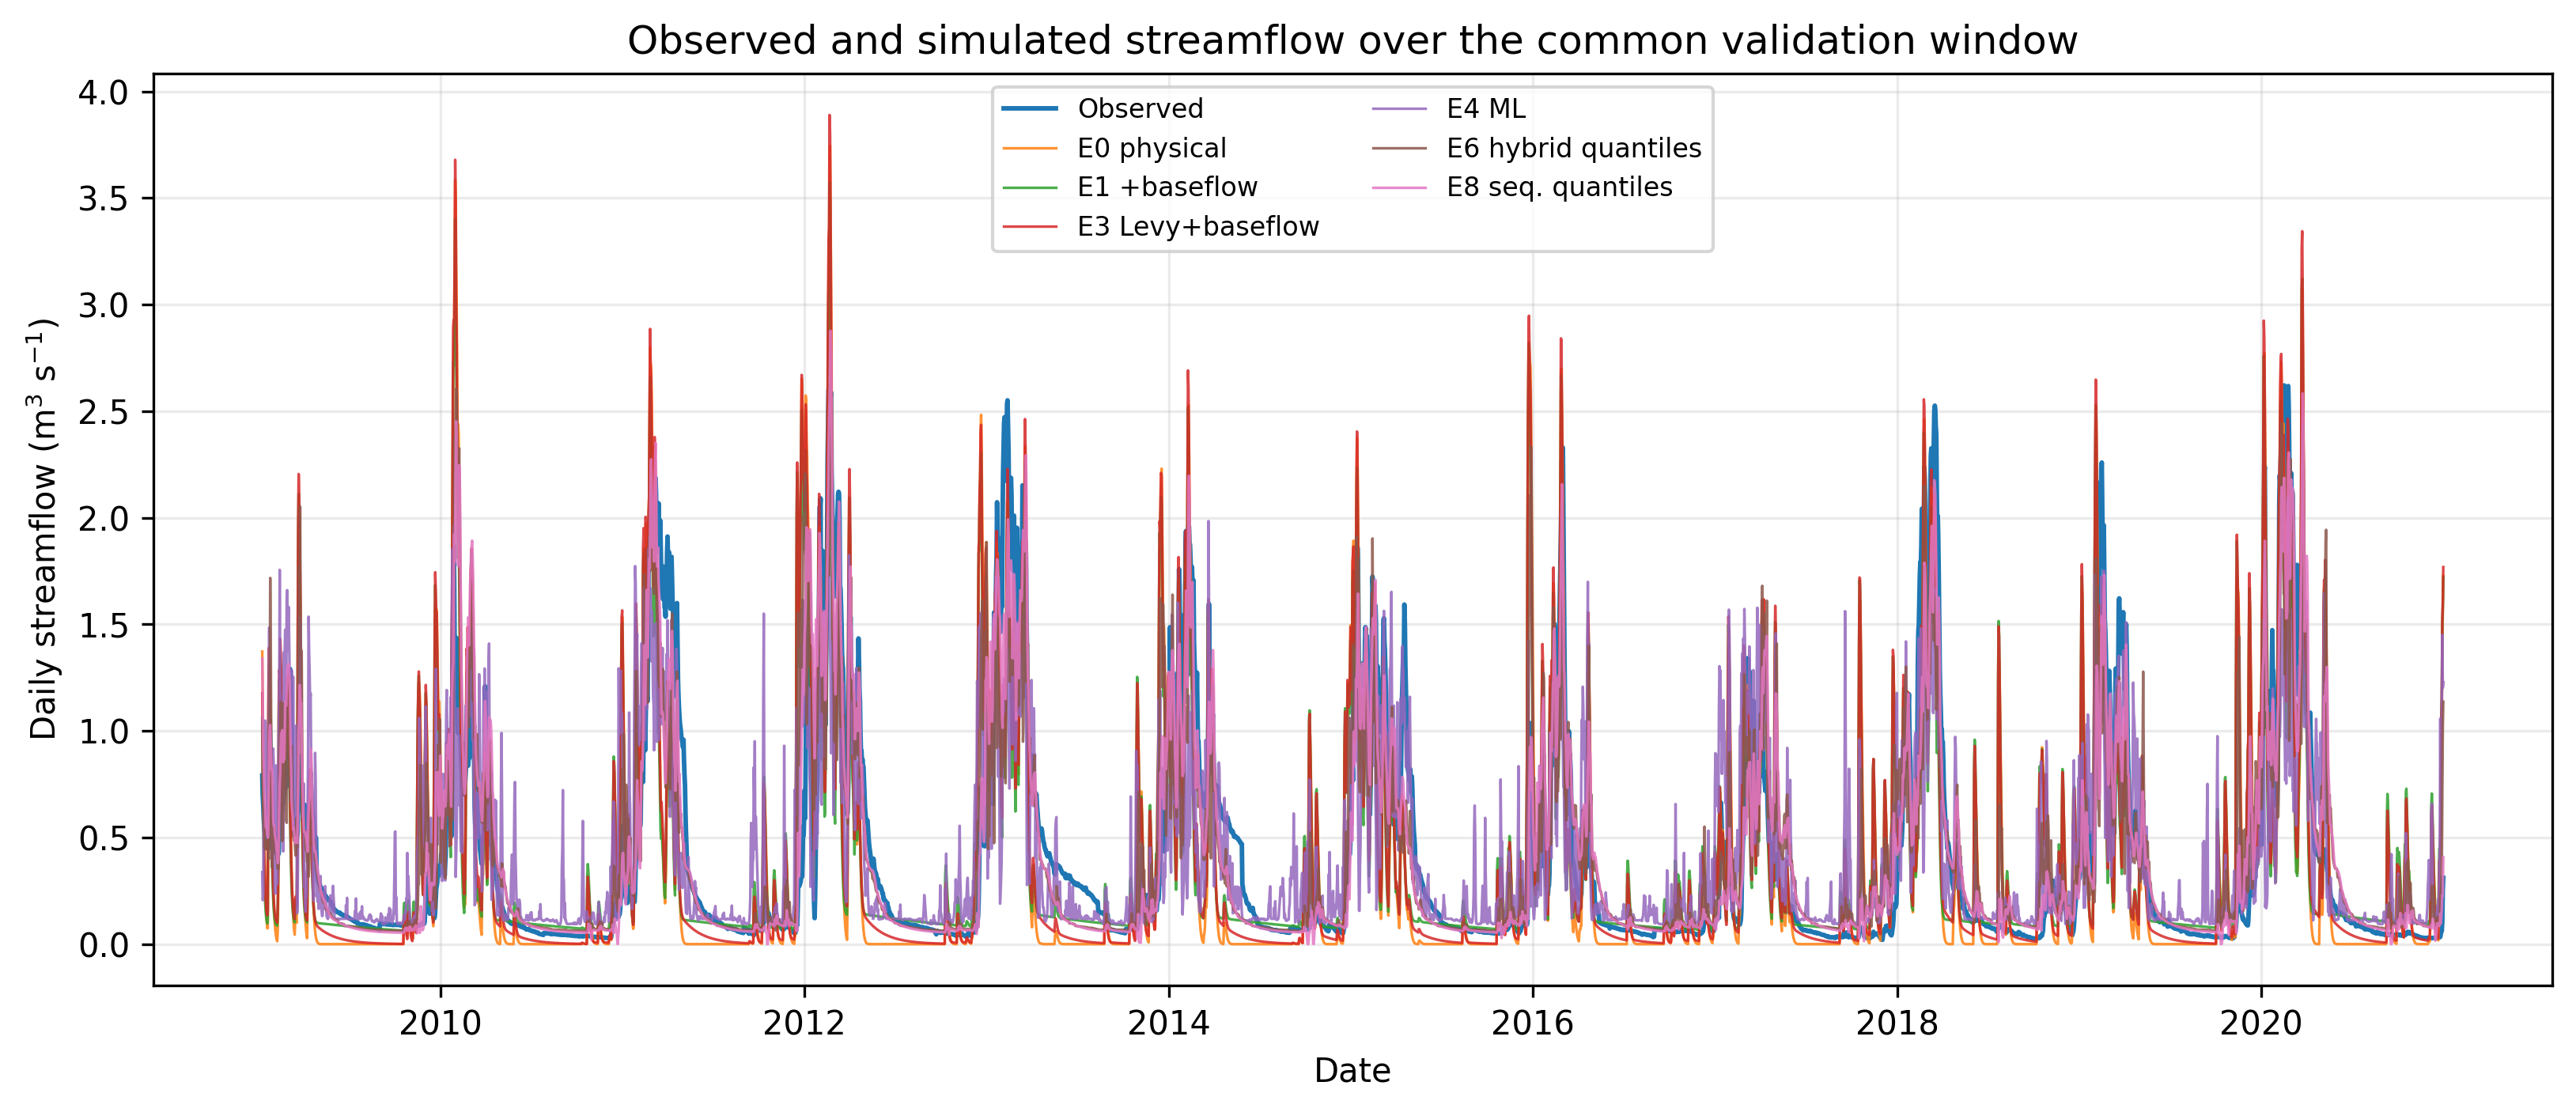
\includegraphics[width=0.98\textwidth]{figures/hydrograph_validation_common.png}
\caption{Observed and simulated daily discharge over the common
validation window for representative physical, pure ML and hybrid
models.}
\label{fig:hydrograph-common}
\end{figure*}

\begin{figure}[t]
\centering
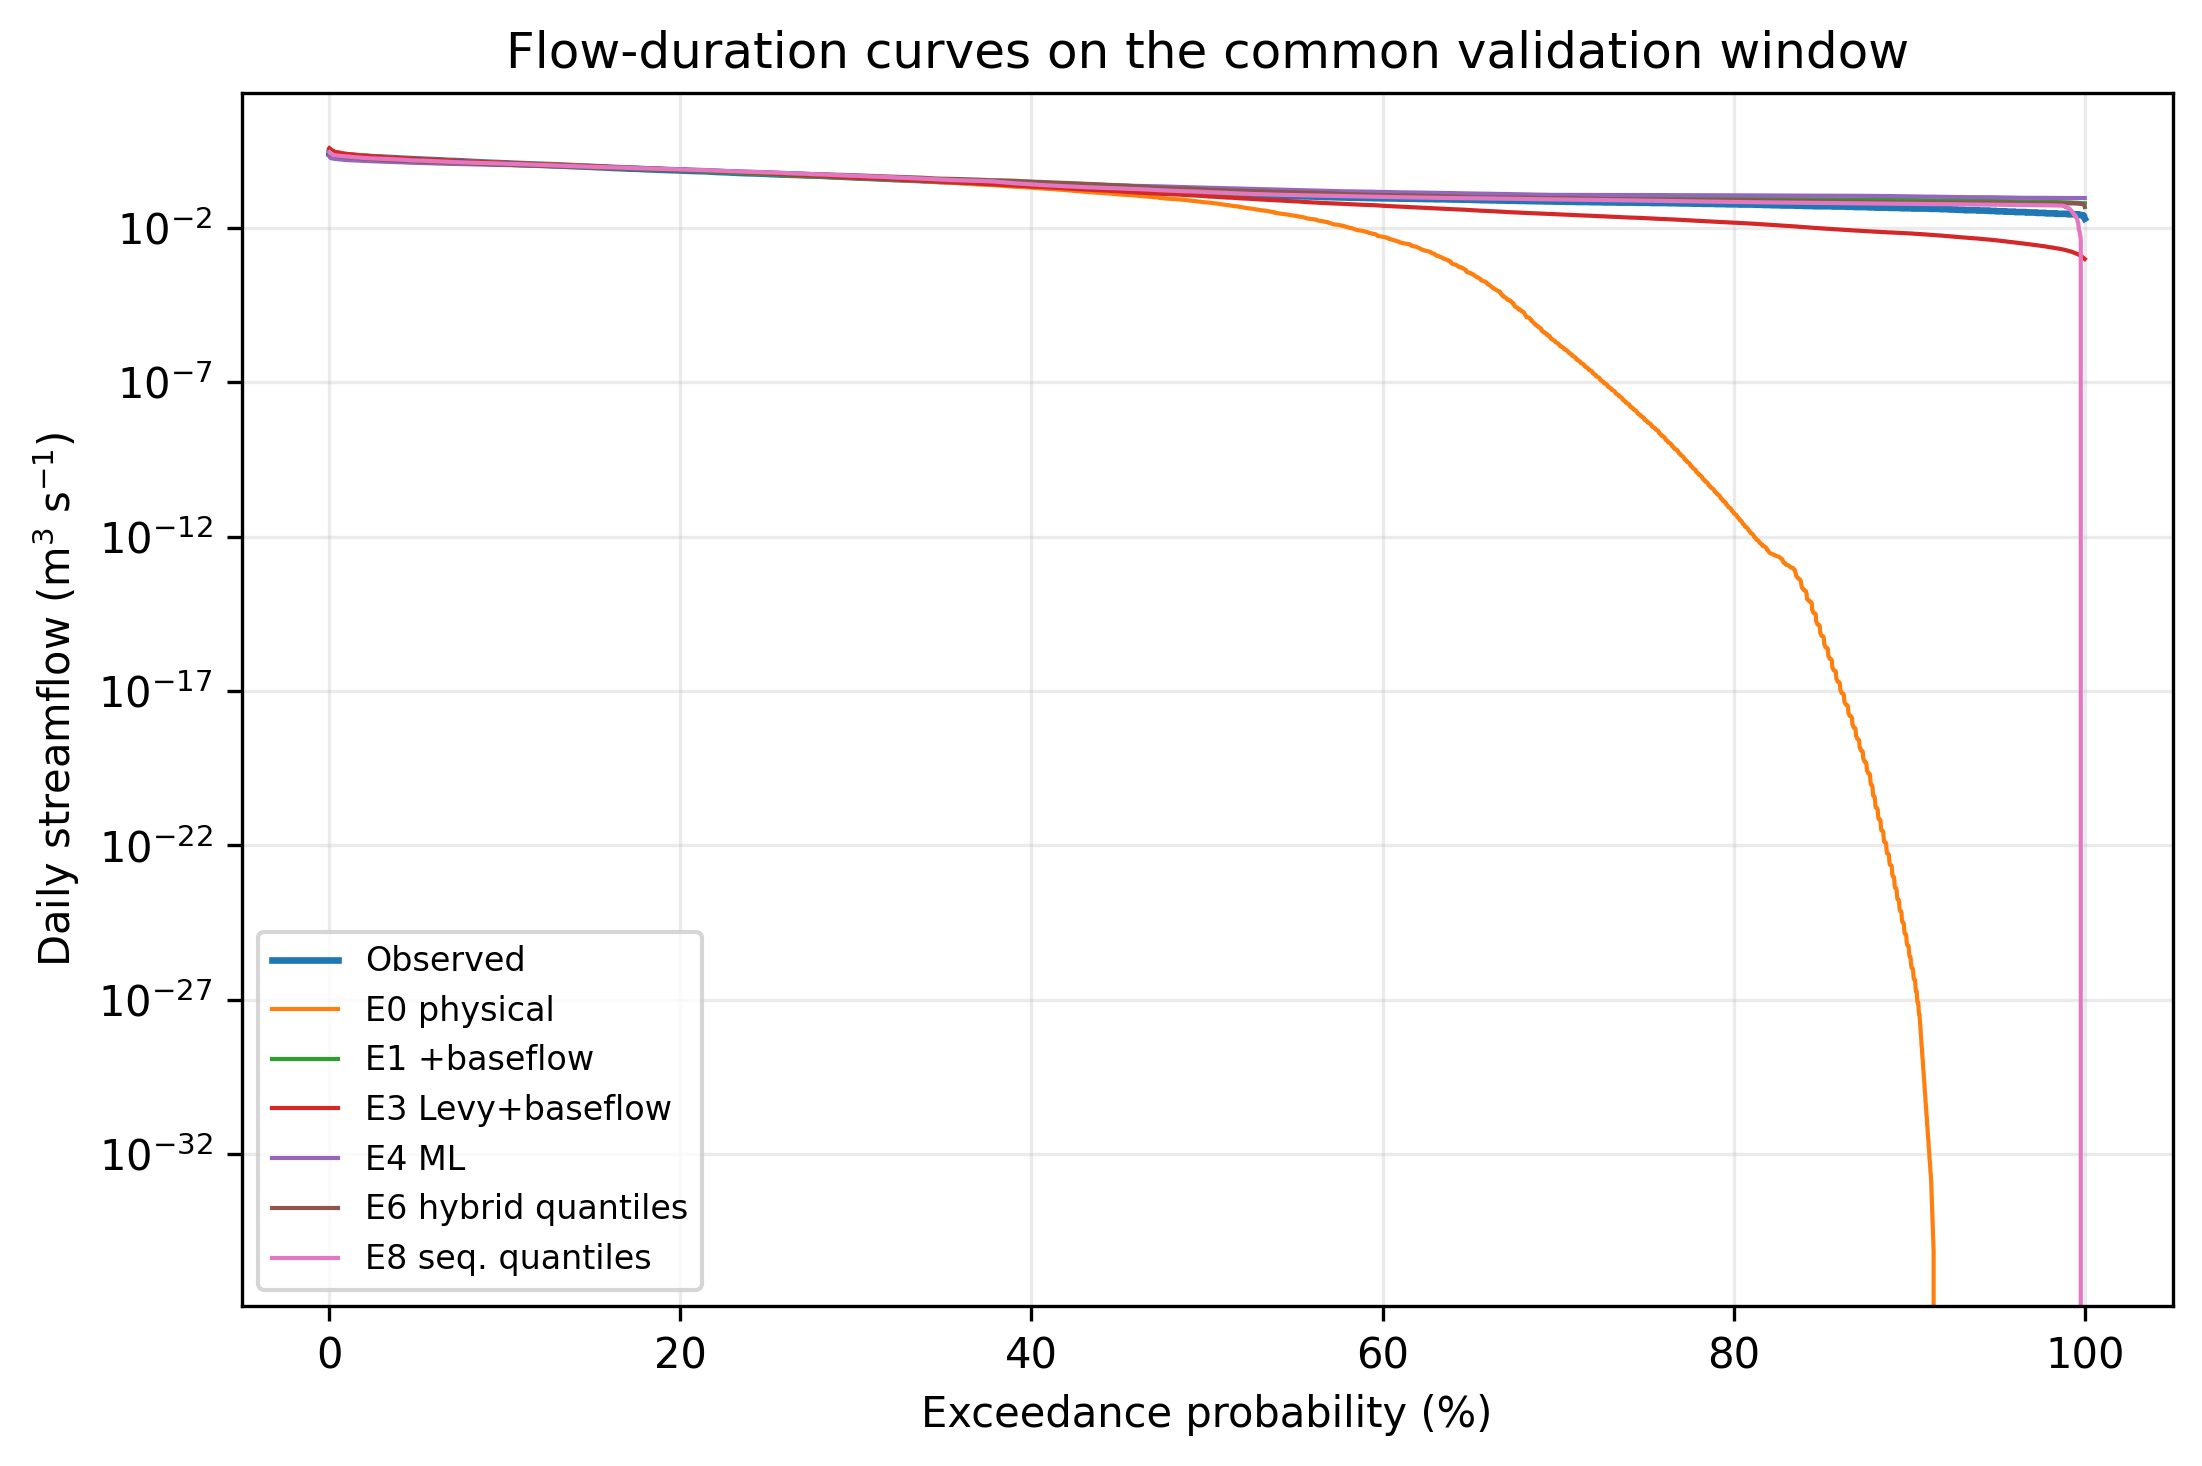
\includegraphics[width=0.95\linewidth]{figures/fdc_common.png}
\caption{Flow-duration curves for observed discharge and representative
simulations over the common validation window.}
\label{fig:fdc-common}
\end{figure}

\subsection{Ablation effects}\label{subsec:ablation-results}

The ablation contrasts in Table~\ref{tab:ablation} and
Fig.~\ref{fig:ablation-effects} quantify the incremental contribution
of each modelling component. Adding the baseflow reservoir to the
deterministic physical model (E1--E0) increased NSE by 0.024 and
reduced RMSE by 0.009~m$^3$\,s$^{-1}$. Under stochastic forcing,
the baseflow effect was smaller but remained positive in NSE and KGE
(E3--E2). The direct addition of L\'{e}vy perturbations under active
baseflow (E3--E1) had mixed effects: NSE decreased by 0.010 while KGE
improved by 0.011, confirming that L\'{e}vy noise does not
consistently improve point predictions.

The largest robust improvement came from hybridization. Replacing the
physical mean output with the quantile-based hybrid (E6--E3) increased
NSE by 0.311 and reduced RMSE by 0.133~m$^3$\,s$^{-1}$, a gain
comparable to the 23--27\% NSE improvements reported by
\citet{yang2020} when ML surrogates were enriched with synthetic
physical data. The quantile-versus-mean contrast (E6--E5) added 0.114
NSE and 0.095 KGE, isolating the information value of distributional
descriptors beyond the ensemble mean alone.

\begin{table*}[t]
\caption{Ablation effects on the common validation window. Positive
$\Delta$NSE and $\Delta$KGE indicate improvement; negative
$\Delta$RMSE and $\Delta$MAE indicate error reduction.}
\label{tab:ablation}
\centering
\small
\begin{tabular*}{\textwidth}{@{\extracolsep{\fill}}llllrrrr@{}}
\toprule
Ablation & Baseline & Candidate
  & $\Delta$NSE & $\Delta$KGE & $\Delta$RMSE & $\Delta$MAE \\
\midrule
deterministic\_baseflow
  & E0\_RAMIS\_DET\_NOBF & E1\_RAMIS\_DET\_BF
  & 0.024 & 0.000 & -0.009 & -0.022 \\
stochastic\_baseflow
  & E2\_RAMIS\_LEVY\_NOBF & E3\_RAMIS\_LEVY\_BF
  & 0.002 & 0.008 & -0.001 & -0.012 \\
levy\_given\_baseflow
  & E1\_RAMIS\_DET\_BF & E3\_RAMIS\_LEVY\_BF
  & -0.010 & 0.011 & 0.004 & 0.008 \\
pure\_ml\_vs\_physical
  & E3\_RAMIS\_LEVY\_BF & E4\_ML\_PURE\_XGB
  & 0.147 & -0.064 & -0.056 & -0.033 \\
hybrid\_mean\_vs\_physical
  & E3\_RAMIS\_LEVY\_BF & E5\_HYB\_XGB\_MEAN
  & 0.198 & -0.010 & -0.078 & -0.046 \\
hybrid\_quantiles\_vs\_physical
  & E3\_RAMIS\_LEVY\_BF & E6\_HYB\_XGB\_QUANTILES
  & 0.311 & 0.085 & -0.133 & -0.094 \\
quantiles\_vs\_mean\_xgb
  & E5\_HYB\_XGB\_MEAN & E6\_HYB\_XGB\_QUANTILES
  & 0.114 & 0.095 & -0.055 & -0.048 \\
gru\_mean\_vs\_xgb\_mean
  & E5\_HYB\_XGB\_MEAN & E7\_HYB\_GRU\_MEAN
  & 0.060 & 0.074 & -0.028 & -0.018 \\
gru\_quantiles\_vs\_xgb\_quantiles
  & E6\_HYB\_XGB\_QUANTILES & E8\_HYB\_GRU\_QUANTILES
  & 0.109 & 0.089 & -0.066 & -0.038 \\
\bottomrule
\end{tabular*}
\end{table*}

\begin{figure}[t]
\centering
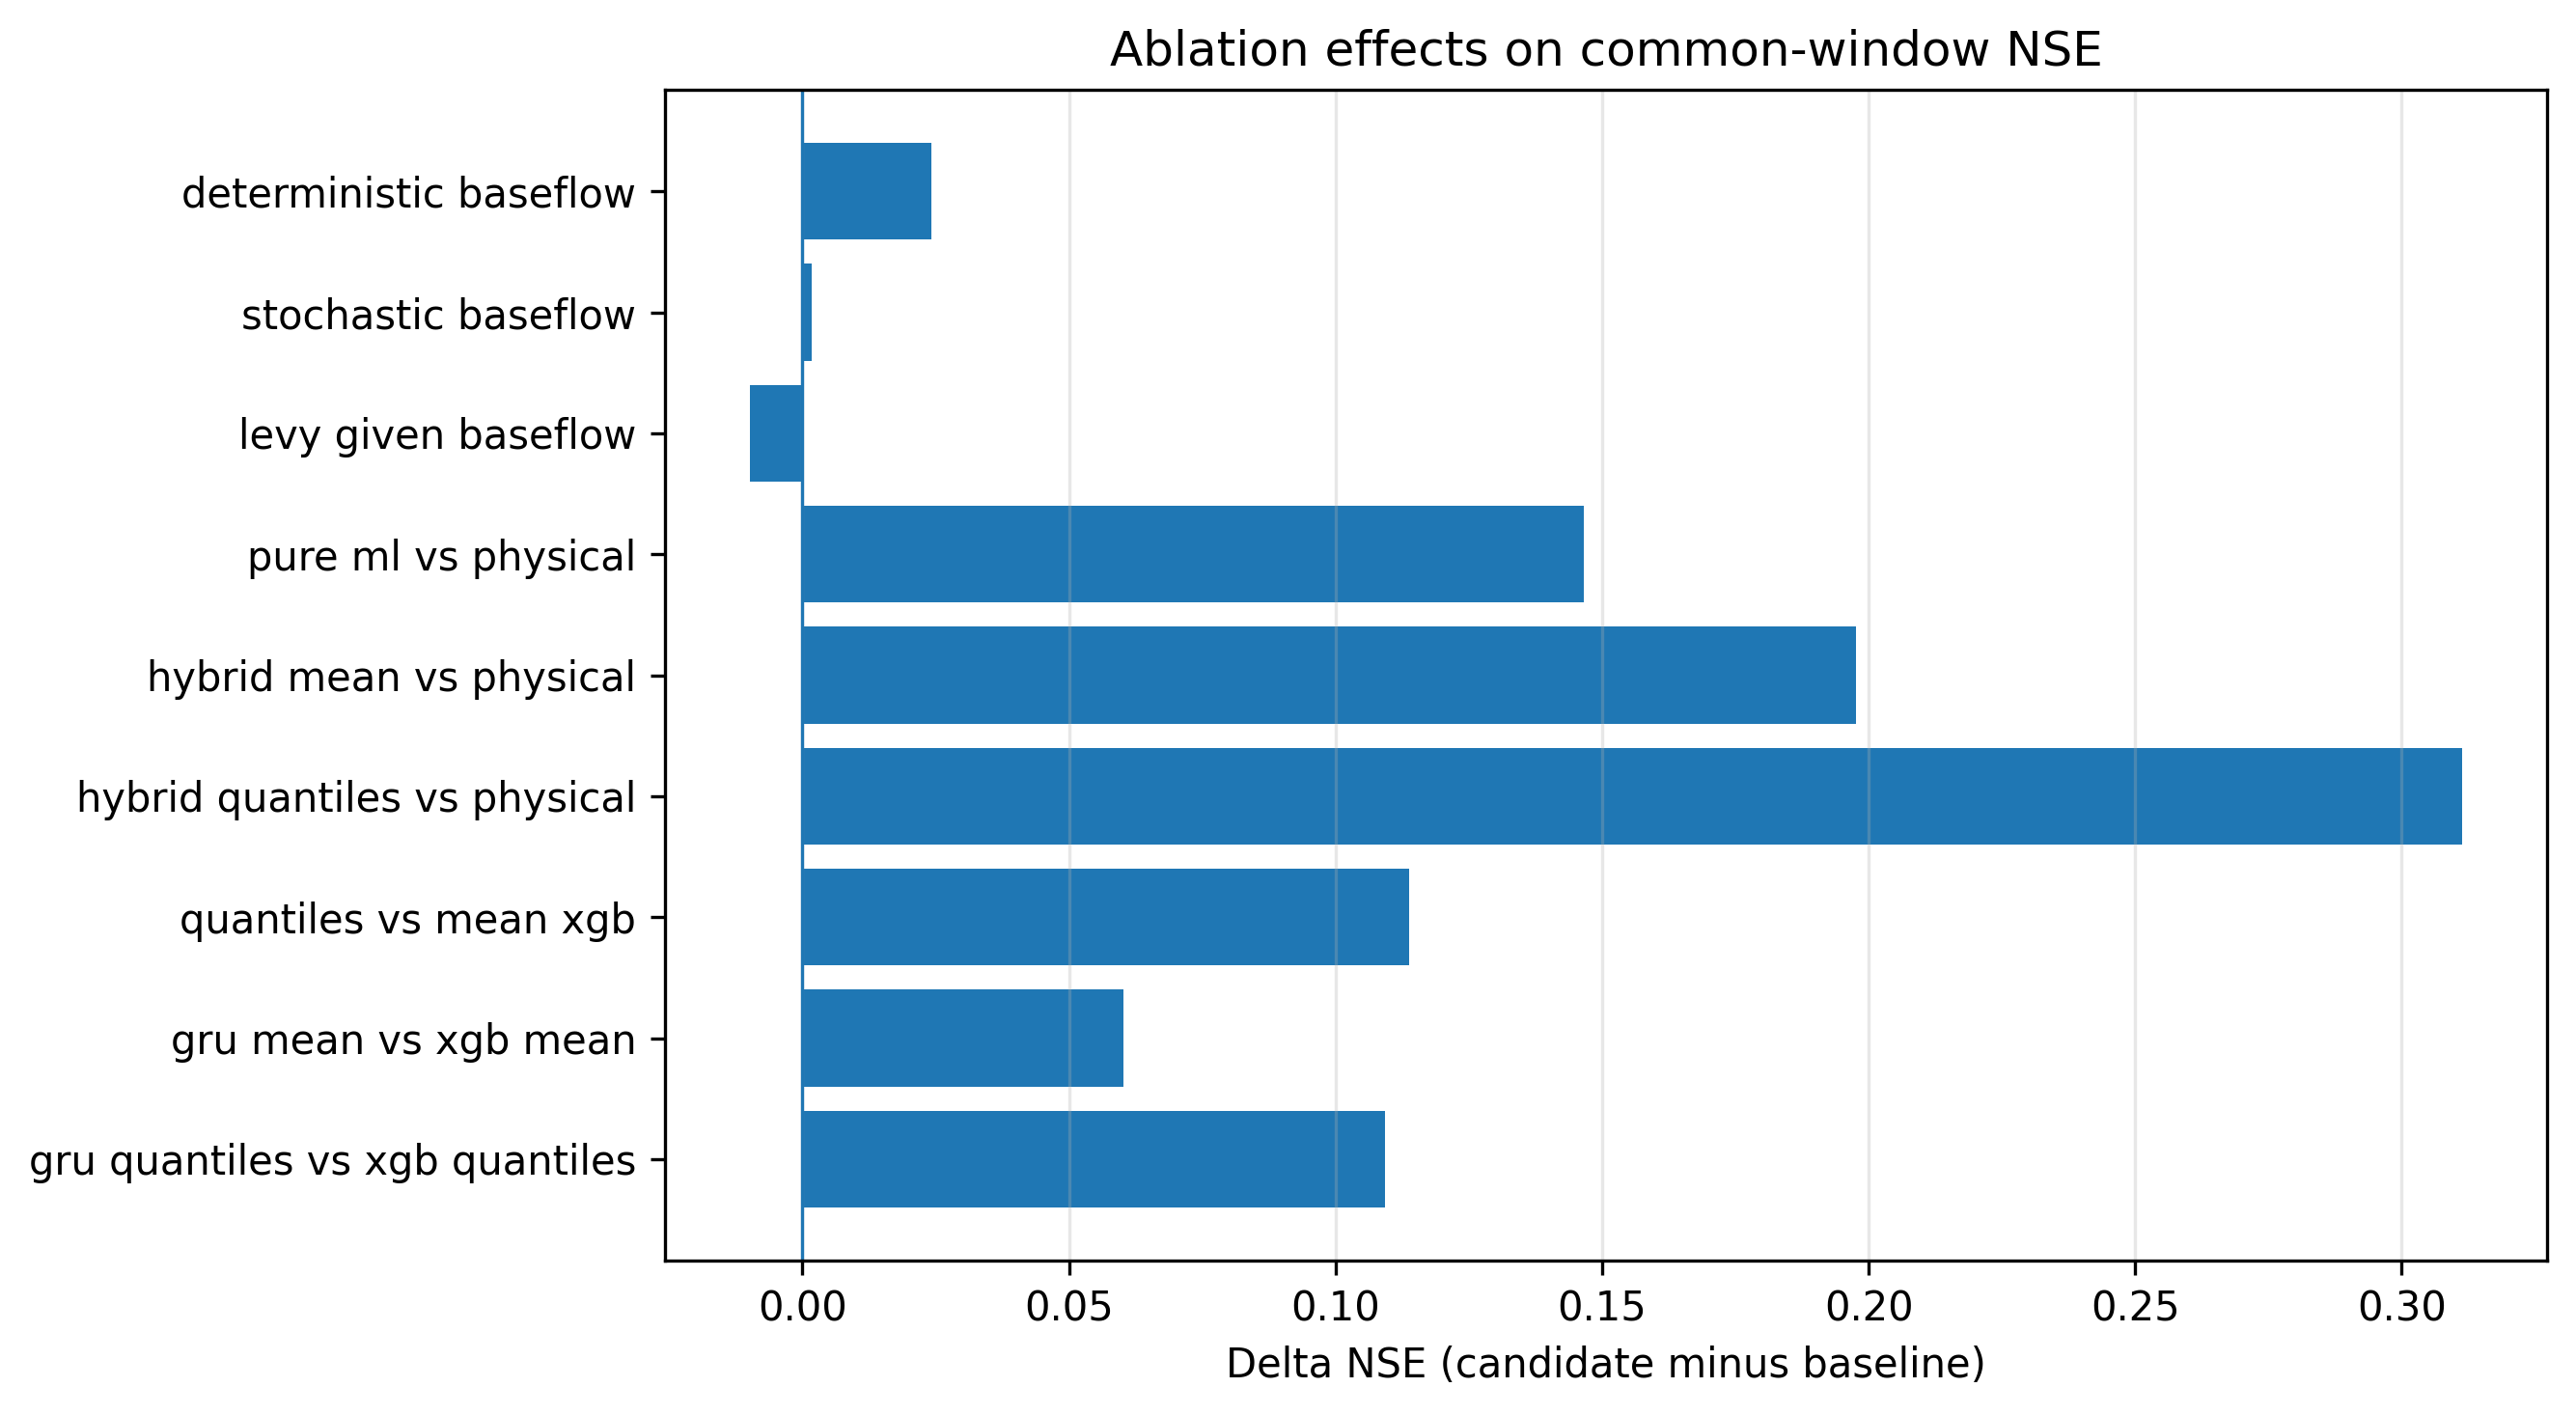
\includegraphics[width=0.95\linewidth]{figures/ablation_effects.png}
\caption{Ablation effects expressed as candidate-minus-baseline
$\Delta$NSE. Numerical values are reported in Table~\ref{tab:ablation}.}
\label{fig:ablation-effects}
\end{figure}

\subsection{Performance by flow regime}\label{subsec:regime-results}

Regime-specific results (Table~\ref{tab:regime-rmse},
Fig.~\ref{fig:regime-rmse}) show that performance is strongly
flow-dependent. Low-flow NSE values were negative for all selected
models, which is expected when the observed variance within the regime
is small \citep{pushpalatha2012}. This reflects a known structural
limitation: the NSE criterion is dominated by variance at the highest
flows, making it an unreliable indicator of skill in the dry season
\citep{pushpalatha2012,van2013}. However, absolute-error metrics
improved markedly with hybridization: low-flow RMSE decreased from
0.177~m$^3$\,s$^{-1}$ (E0) to 0.075~m$^3$\,s$^{-1}$ (E6) and
0.047~m$^3$\,s$^{-1}$ (E8). The improvement in low flows from the
quantile hybrid is consistent with the finding of \citet{lees2021}
that LSTM-based models ``show a large performance improvement for
low-flow bias score (\%BiasFLV)'' relative to conceptual models, and
with \citet{li2024process} who found that physically informed
architectures significantly enhance low-flow simulations. For high
flows, E8 reached the best regime RMSE among the selected models;
the remaining gap at high flows---0.352~m$^3$\,s$^{-1}$ for E8
versus 0.615~m$^3$\,s$^{-1}$ for E0---reflects both the difficulty
of extreme events and the benefit of ensemble quantile features in
capturing the asymmetry of the upper tail.

\begin{table}[t]
\caption{RMSE (m$^3$\,s$^{-1}$) by flow regime for representative
models. Regime thresholds were estimated from calibration observations
only.}
\label{tab:regime-rmse}
\centering
\small
\begin{tabular*}{\linewidth}{@{\extracolsep{\fill}}lrrr@{}}
\toprule
Experiment & Low & Mid & High \\
\midrule
E0\_RAMIS\_DET\_NOBF   & 0.177 & 0.392 & 0.615 \\
E1\_RAMIS\_DET\_BF     & 0.197 & 0.365 & 0.613 \\
E3\_RAMIS\_LEVY\_BF    & 0.185 & 0.387 & 0.604 \\
E4\_ML\_PURE\_XGB      & 0.189 & 0.276 & 0.566 \\
E6\_HYB\_XGB\_QUANTILES & 0.075 & 0.222 & 0.461 \\
E8\_HYB\_GRU\_QUANTILES & 0.047 & 0.171 & 0.352 \\
\bottomrule
\end{tabular*}
\end{table}

\begin{figure}[t]
\centering
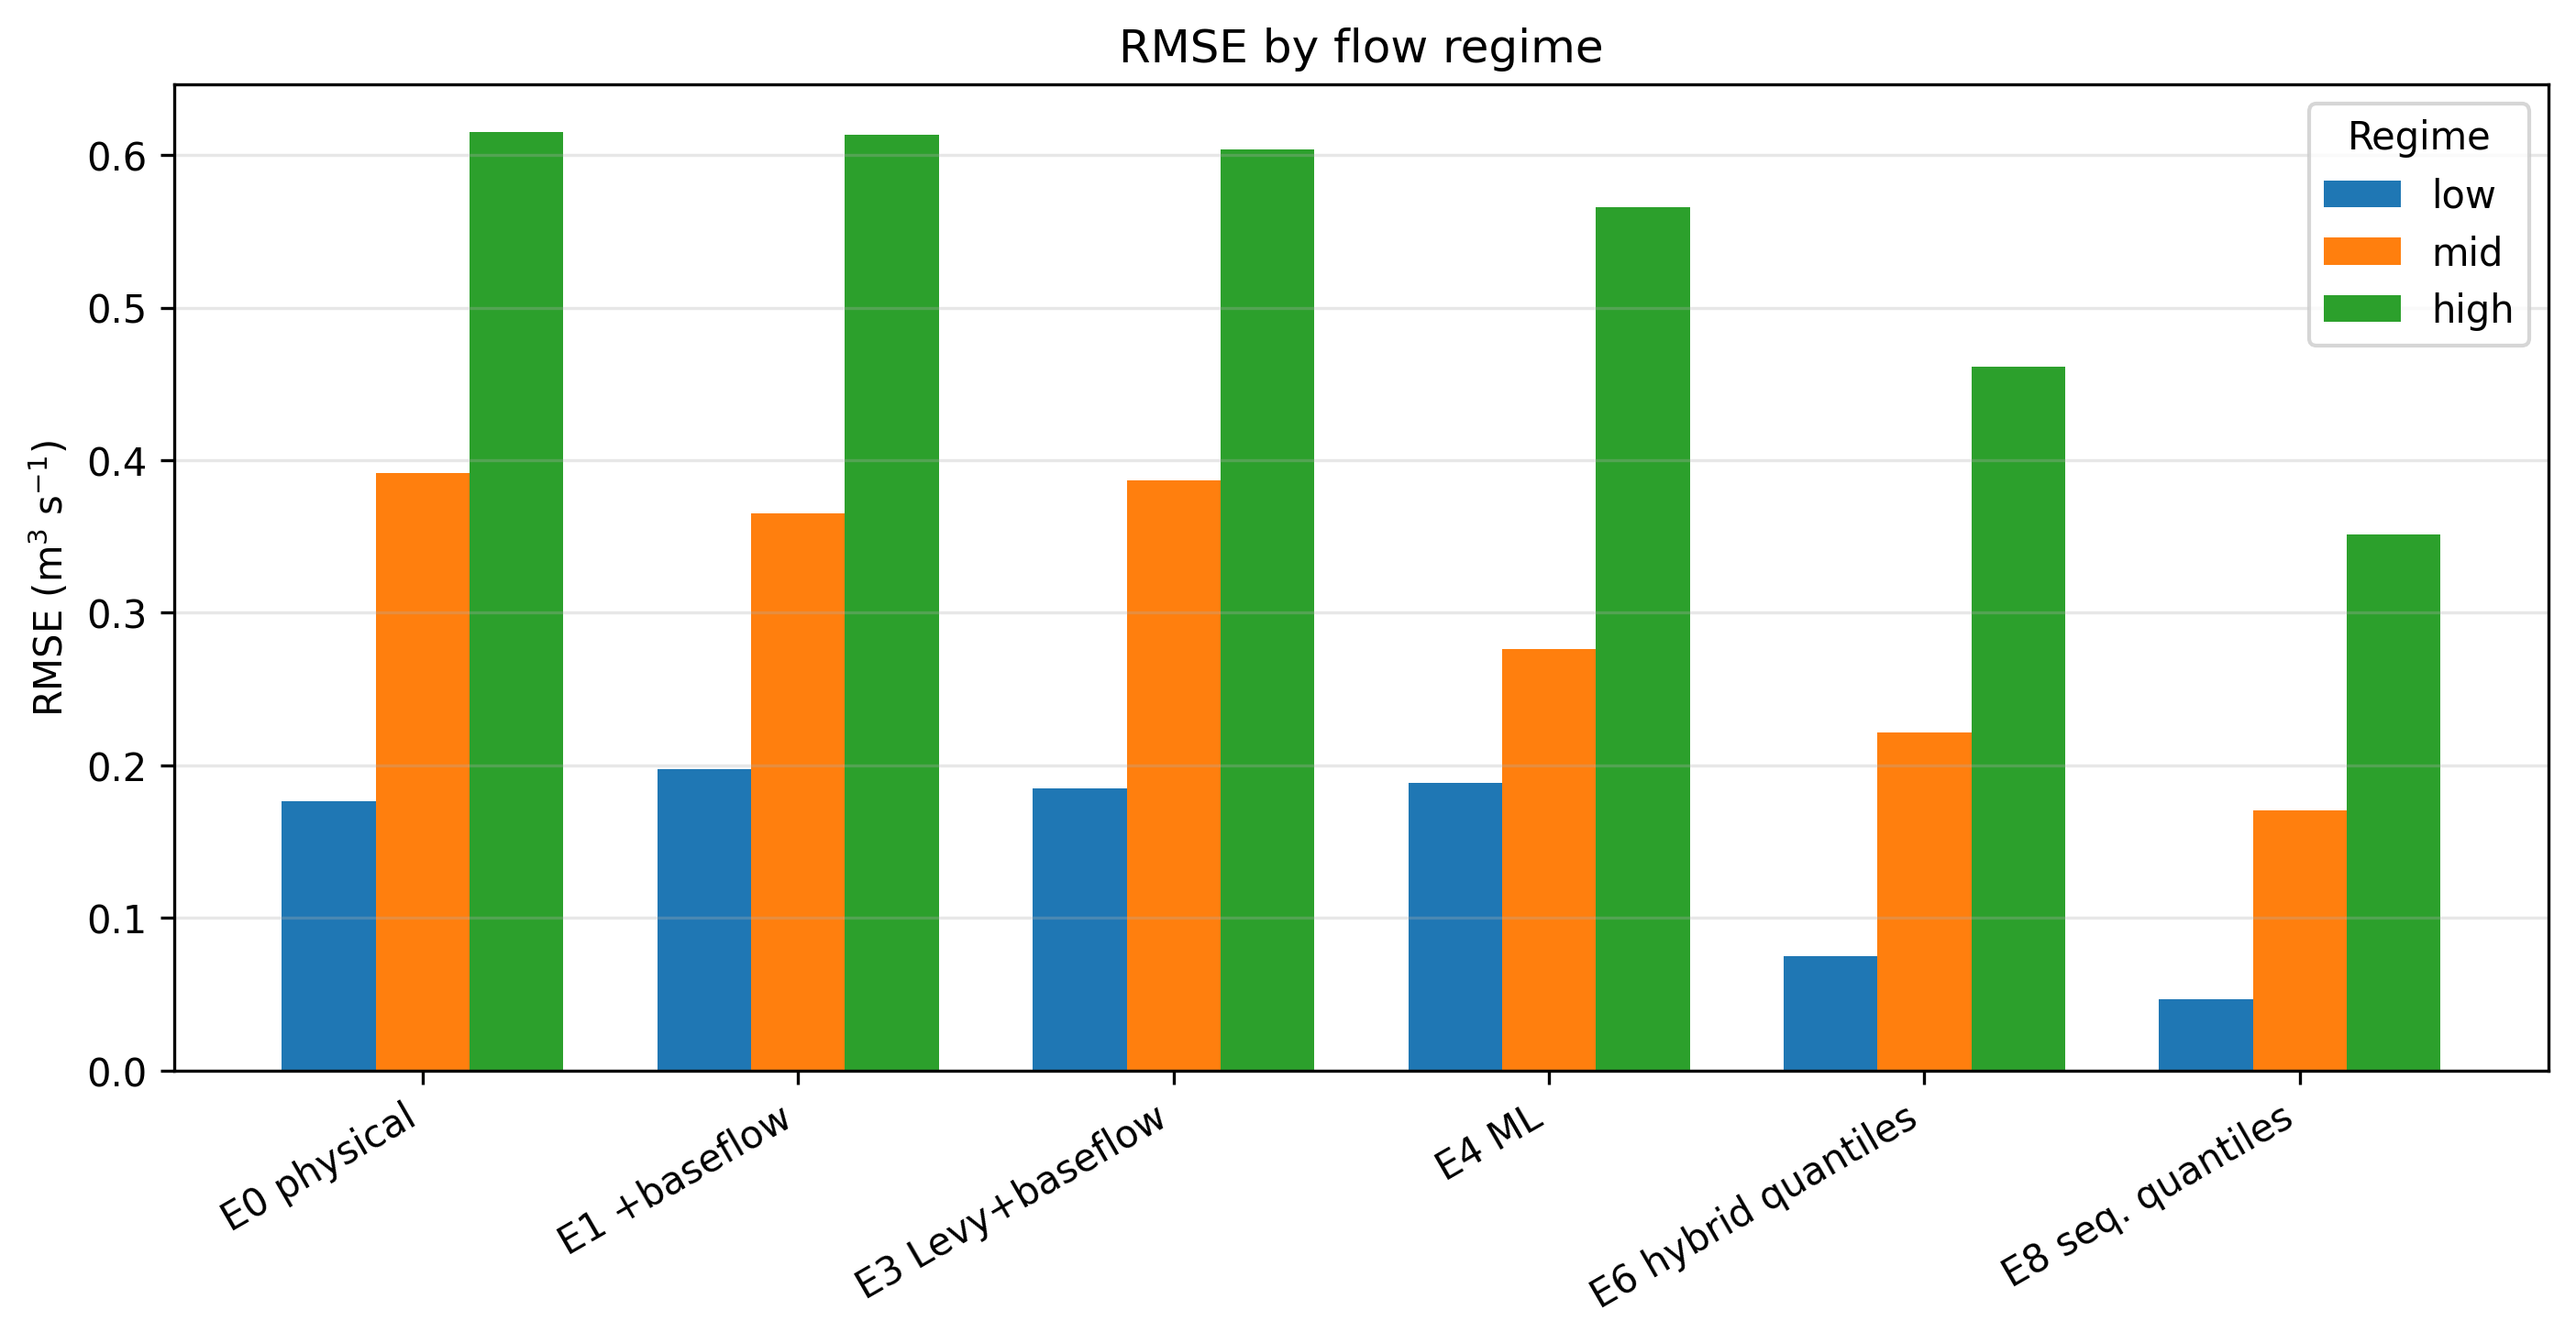
\includegraphics[width=0.95\linewidth]{figures/regime_rmse.png}
\caption{RMSE by low, mid and high flow regimes for representative
models. Values correspond to Table~\ref{tab:regime-rmse}.}
\label{fig:regime-rmse}
\end{figure}

\subsection{Uncertainty diagnostics and backend audit}
\label{subsec:uncertainty-results}

The stochastic physical bands were strongly underdispersive
(Table~\ref{tab:uncertainty}, Fig.~\ref{fig:uncertainty-diagnostics}).
E2 achieved PICP\,=\,0.160 and E3 achieved PICP\,=\,0.004, far below
the nominal 0.95 target, with correspondingly high Winkler scores.
These results confirm what \citet{abaza2017} described as the
predominant failure mode of hydrological ensemble prediction systems:
``most hydrological ensemble prediction systems fail to account for
all sources of uncertainty, leading to under-dispersed forecasts.''
The stochastic bands should therefore be interpreted as physically
structured stochastic references rather than calibrated predictive
intervals \citep{crochemore2016,thiboult2016}.

Backend metadata are summarized in Table~\ref{tab:backend}. The
XGB-labelled experiments (E4--E6) used \texttt{sklearn\_hgb}, and
the GRU-labelled experiments (E7, E8) used
\texttt{fallback\_mlp\_on\_flattened\_sequences}. The reproducibility
checklist (Table~\ref{tab:reproducibility}) returned WARN for
anti-leakage and physical audits but no FAIL. WARN items were
associated with missing observed-flow values, low-flow physical
limitations and backend caveats, not with direct evidence of temporal
leakage.

\begin{table}[t]
\caption{Uncertainty diagnostics for stochastic physical reference
bands.}
\label{tab:uncertainty}
\centering
\small
\begin{tabular*}{\linewidth}{@{\extracolsep{\fill}}lrrrr@{}}
\toprule
Experiment & PICP & PINAW & MPIW & Winkler \\
\midrule
E2\_RAMIS\_LEVY\_NOBF & 0.160 & 0.084 & 0.219 & 7.297 \\
E3\_RAMIS\_LEVY\_BF   & 0.004 & 0.003 & 0.009 & 10.050 \\
\bottomrule
\end{tabular*}
\end{table}

\begin{figure}[t]
\centering
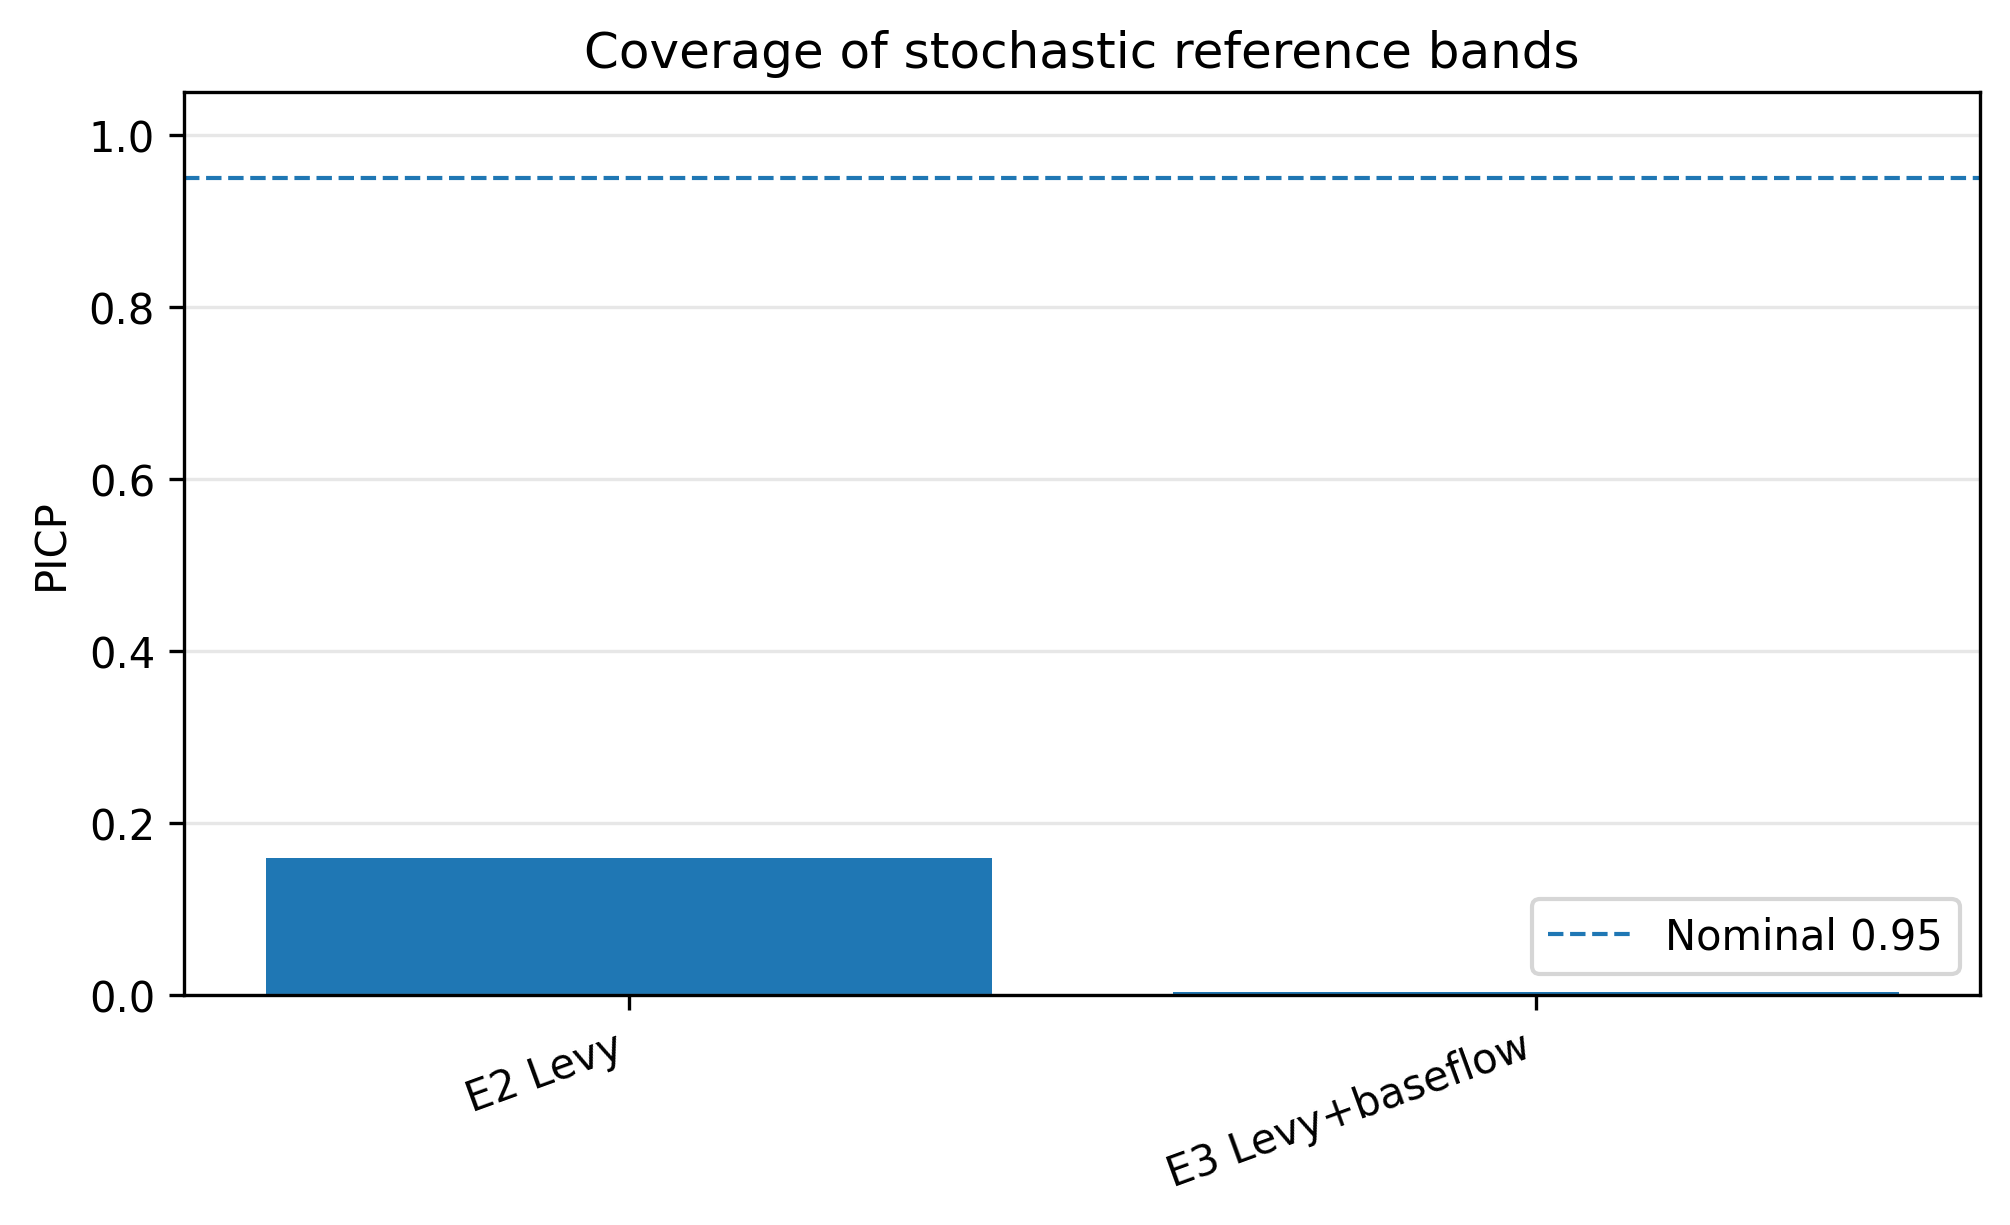
\includegraphics[width=0.95\linewidth]{figures/uncertainty_diagnostics.png}
\caption{Prediction interval coverage probability for stochastic
physical references. The dashed line marks the nominal 0.95 target.}
\label{fig:uncertainty-diagnostics}
\end{figure}

\begin{table*}[t]
\caption{Backend-aware manuscript notes for ML and hybrid configurations.}
\label{tab:backend}
\centering
\small
\begin{tabular*}{\textwidth}{@{\extracolsep{\fill}}lllll@{}}
\toprule
Experiment & ML label & Backend label & Feature source
  & Manuscript claim \\
\midrule
E4\_ML\_PURE\_XGB      & xgboost & sklearn\_hgb & observed\_forcing
  & report as gradient boosting (HGB) \\
E6\_HYB\_XGB\_QUANTILES & xgboost & sklearn\_hgb & stochastic\_ensemble
  & report as gradient boosting (HGB) \\
E7\_HYB\_GRU\_MEAN     & gru & fallback\_mlp\_on\_flattened\_sequences
  & stochastic\_ensemble & fallback MLP, not real recurrent GRU \\
E8\_HYB\_GRU\_QUANTILES & gru & fallback\_mlp\_on\_flattened\_sequences
  & stochastic\_ensemble & fallback MLP, not real recurrent GRU \\
\bottomrule
\end{tabular*}
\end{table*}

\begin{table*}[t]
\caption{Reproducibility checklist for the current evidence package.}
\label{tab:reproducibility}
\centering
\small
\begin{tabular*}{\textwidth}{@{\extracolsep{\fill}}lll@{}}
\toprule
Item & Status & Evidence \\
\midrule
Common validation intersection & PASS
  & leaderboard\_common\_intersection.csv \\
Anti-leakage audit & WARN & leakage\_audit\_status.txt=WARN \\
Physical audit   & WARN & physical\_audit\_status.txt=WARN \\
Figure manifest  & PASS
  & outputs/figures/phase34/phase34\_figure\_manifest.csv \\
GRU wording      & WARN & E7/E8 use fallback backend \\
Optional physical components in figures & WARN
  & skipped entries in phase34\_figure\_manifest.csv \\
\bottomrule
\end{tabular*}
\end{table*}

%% =====================================================================
%% 4. DISCUSSION
%% =====================================================================
\section{Discussion}\label{sec:discussion}

\subsection{Hydrological memory and the role of baseflow}
\label{subsec:discussion-baseflow}

The positive deterministic contrast E1--E0 confirms that adding a
linear baseflow reservoir improves the physical RAMIS baseline, in
agreement with the modelling evidence from semi-arid Andean catchments
reviewed by \citet{nauditt2017}: ``the best simulations could be
achieved with separate parameter sets for varying hydro-climatic
conditions,'' and a dedicated slow-drainage component is necessary to
represent the recession-dominated dry season. The NSE and RMSE
improvements are modest in absolute terms but hydrologically
meaningful: the baseflow reservoir introduces the delayed drainage
memory that cannot be captured by an instantaneous fast-flow response
alone. This conclusion echoes the quantitative demonstration of
\citet{adnan2021comparison} that including runoff memory in model
inputs is ``appropriate and contributes to an improvement of the models'
accuracy.''

However, the regime results in Table~\ref{tab:regime-rmse} show that
low-flow simulation remains challenging despite the presence of the
baseflow reservoir. A single linear store can represent average
recession behaviour but is insufficient when the storage is
heterogeneous across the catchment, as would be expected in an
Altiplano landscape with wetlands, peatlands (bofedales) and variable
permeability \citep{harman2009}. \citet{harman2009} showed
theoretically that ``between-hillslope heterogeneity alone can give
rise to apparently nonlinear recession slope curves,'' implying that
the effective storage--discharge relationship inferred from recession
analysis will always appear more complex than a simple linear
reservoir. A practical consequence for StoHyMoLAP is that the
baseflow improvement is bounded by the structural limitation of a
single-reservoir representation. This is consistent with the finding
of \citet{van2013} that ``parallel reservoirs with independent time
constants increase model performance in groundwater-dominated
catchments,'' suggesting a natural extension for future work.

The limited low-flow improvement also reflects a fundamental
measurement challenge: the NSE criterion assigns most weight to
high-flow variance \citep{pushpalatha2012}, so the global NSE
improvement from the baseflow reservoir is modest even when the
absolute error in the low-flow regime is reduced. Following the
recommendation of \citet{pushpalatha2012} to use the NSE on inverse
flows (NSE$^*_{iQ}$) to focus evaluation on the lowest 20\% of
flows, future studies should track this metric explicitly in addition
to global NSE.

\subsection{L\'{e}vy perturbations as stochastic descriptors rather
than calibrated uncertainty}\label{subsec:discussion-levy}

L\'{e}vy perturbations modify the distributional behaviour of physical
simulations and, in principle, can represent the heavy-tailed
variability documented for Andean precipitation and streamflow. The
coverage diagnostics in Table~\ref{tab:uncertainty}, however,
demonstrate that the resulting stochastic bands are strongly
underdispersive: PICP values of 0.16 and 0.004 are far below the
nominal 0.95, and Winkler scores reflect large penalties for missing
observations. This failure to achieve calibrated coverage is not
unique to L\'{e}vy-driven models: \citet{thiboult2016} showed that
even sophisticated multi-model ensemble systems ``fail to maintain
the required dispersion throughout the entire forecast horizon,'' and
\citet{crochemore2016} found that correcting precipitation inputs
alone is ``obviously not enough to achieve streamflow forecast
reliability.'' The more general point is that calibrated uncertainty
requires explicitly accounting for all sources of error
simultaneously---not only stochastic forcing, but also parameter
uncertainty, structural uncertainty and initial-condition uncertainty
\citep{demirel2013,thiboult2016}.

The underdispersive nature of the bands does not negate the value of
L\'{e}vy perturbations within StoHyMoLAP; it merely redirects that
value. Rather than serving as calibrated intervals, the stochastic
ensemble summaries---particularly the quantile descriptors in
Eq.~\ref{eq:quantiles}---function as informative features that encode
distributional information about the conditional response of the
physical model. The key insight from \citet{gabellani2007} is directly
applicable here: ``the spectral slopes of the rain fields play an
essential role in determining the hydrological response,'' and features
that preserve asymmetry and tail behaviour (quantiles) carry more
information than features that collapse the distribution to its mean.
\citet{swiderski2016} showed that quantile representations are
``less sensitive to fat-tailed distributions and outliers,'' a
property that is particularly desirable when the ensemble members are
driven by $\alpha$-stable noise.

\subsection{Why quantile-based hybridization works}
\label{subsec:discussion-hybrid}

The most robust empirical signal in this study is the advantage of
quantile-based hybridization. The E6--E5 contrast adds 0.114 NSE and
0.095 KGE purely from switching the physical descriptor from a mean
to a quantile vector, holding everything else constant. This result
is interpretable within the framework of \citet{papacharalampous2022}:
``there are two ways for improving predictive performance---improving
the prediction algorithm and discovering new informative predictors,''
and quantile descriptors of the physical ensemble constitute precisely
the latter. A single ensemble mean retains first-moment information
but discards the conditional spread, asymmetry and tail behaviour of
the physical simulation. In the Ramis basin, where the flow regime
alternates sharply between wet-season peaks and dry-season recession,
these distributional properties are not constant: the upper quantiles
expand during the wet season while the lower quantiles collapse. This
asymmetric dynamics is informationally invisible to a mean-only
descriptor and yet is directly observable in the quantile vector.

The hybrid emulator (E6) also outperforms the pure ML baseline (E4)
despite E4 having access to observed meteorological forcing. This
indicates that physically simulated ensemble descriptors provide
information beyond what is contained in the observed forcings alone, a
result consistent with \citet{yang2020} who found NSE improvements of
23\% when ML surrogates were enriched with synthetic physical data, and
with \citet{mekonnen2015} who showed that SWAT outputs ``provide a
proxy about the instantaneous wetness condition of the catchment.''
The interpretation is that the physical ensemble descriptors
effectively encode catchment antecedent state in a form that the ML
emulator can more readily exploit than raw meteorological time series.
This is consistent with the argument of \citet{moreido2021} that ``a
machine learning model needs a teacher (hydrologist) that provides it
with textbooks and then leaves it for self-teaching,'' and with the
finding of \citet{okkan2021} that models lacking antecedent runoff
information cannot compete with physically constrained alternatives.

One should note, however, that the E6 advantage over E4 is partly
confounded with the difference in feature type (ensemble statistics
versus raw forcing), and the E6--E4 contrast alone cannot distinguish
between the value of hydrological structure and the value of temporal
aggregation. Resolving this would require an additional ablation
experiment pairing observed forcing with quantile features derived from
simple lag statistics, which is left for future work. This caveat is
consistent with the general warning of \citet{zhong2023} that
``implicit coupling... requires more elaborate design of the model
structure and inputs, as well as more thorough verification of the
results to avoid learning other misleading relationships.''

\subsection{Backend-aware interpretation of the sequential experiments}
\label{subsec:discussion-backend}

E8 is the top-ranked configuration in Table~\ref{tab:ranking}, but the
result must be interpreted together with Table~\ref{tab:backend}. The
fallback MLP backend in E7 and E8 processes flattened sequences rather
than recurrent hidden states, and therefore does not implement the
temporal gating mechanism that is the defining feature of GRU cells
\citep{cho2014gru,kratzert2018}. The valid conclusion is narrower:
a GRU-labelled sequential hybrid using quantile descriptors and
implemented with a fallback flattened-sequence MLP achieved the best
validation metrics in the current environment. Whether a true recurrent
GRU would reproduce or exceed this performance cannot be established
from the current evidence package.

The consistent ordering of quantile over mean descriptors in both the
XGB-labelled (E6$>$E5) and the GRU-labelled (E8$>$E7) families
suggests that the descriptor choice is the driver of improvement rather
than the emulator architecture. This is an important practical
conclusion: it implies that the gain from quantile hybridization should
be architecture-agnostic, and therefore reproducible under a true GRU
backend. Future work should rerun E7 and E8 with TensorFlow or PyTorch
backends and compare the GRU-specific gain to the descriptor-specific
gain measured here. Transparent backend reporting is essential for such
comparison, as emphasized by \citet{hall2021}: ``open hydrologists
document all components of their data collection and analysis pipeline,
favoring open and non-proprietary technologies.''

\subsection{Leakage, reproducibility and submission readiness}
\label{subsec:discussion-leakage}

The audit status in Table~\ref{tab:reproducibility} strengthens the
comparison by documenting the major leakage controls: strict temporal
splitting, non-negative lags, sequence construction within temporal
subsets, train-only scalers and train-only regime thresholds.
``Only 1\% of hydrology papers were fully reproducible'' in a recent
large-scale survey \citep{hall2021}, and the StoHyMoLAP audit is an
explicit step toward closing that gap.

The WARN status should remain visible in the manuscript or
supplementary material. WARN does not indicate detected temporal
leakage, but it does identify issues that affect interpretation:
missing observed-flow values, physical low-flow limitations,
underdispersive stochastic bands and fallback ML backends. These are
honest disclosures consistent with the open-science principles
advocated by \citet{hall2021} and with the rigorous benchmarking
framework recommended by \citet{papacharalampous2022}.

%% =====================================================================
%% 5. LIMITATIONS
%% =====================================================================
\section{Limitations}\label{sec:limitations}

This study has five main limitations. First, the sequential experiments
labelled as GRU were not executed with a real recurrent backend, so
their results cannot support claims about recurrent neural networks
\citep{kratzert2018}. Second, the L\'{e}vy stochastic bands are
underdispersive and should not be treated as calibrated uncertainty
intervals; recalibration following the guidelines of \citet{thiboult2016}
and \citet{abaza2017} is required before these bands can be used
operationally. Third, low-flow bias remains substantial despite
improvements in absolute-error metrics; future work should apply
the inverse-flow NSE criterion of \citet{pushpalatha2012} to focus
calibration explicitly on the dry-season regime. Fourth, the audit
status is WARN rather than fully PASS, requiring transparent reporting
of missing observations and physical-audit warnings. Fifth, %% [FILL]
confirm data provenance and units (Section~\ref{subsec:study-area}):
if the current package corresponds to an illustrative or
reduced-computation run, or if the discharge series is normalized or
refers to a sub-catchment rather than the full Puente Ramis basin, the
final submission must regenerate the complete evidence package with the
definitive, traceable observed Ramis dataset (source, station, units)
and publication-level calibration settings.

%% =====================================================================
%% 6. CONCLUSIONS
%% =====================================================================
\section{Conclusions}\label{sec:conclusions}

StoHyMoLAP provides a reproducible, audit-controlled framework for
evaluating stochastic physical--machine-learning hybridization in daily
streamflow simulation, applied here to the high-Andean Ramis basin in
the Lake Titicaca system. Four main conclusions emerge from the
controlled ablation.

First, quantile descriptors from the stochastic physical ensemble are
the dominant driver of hybrid improvement: replacing the ensemble mean
with quantile features added 0.114 NSE (E6--E5), and the full
quantile hybrid surpassed the physical model by 0.311 NSE (E6--E3).
This confirms, in an Altiplano setting, the argument of
\citet{papacharalampous2022} and the quantitative demonstration of
\citet{houenafa2025} that distributional descriptors carry information
beyond a single trajectory.

Second, the baseflow reservoir improves the deterministic physical
baseline (E1--E0: $\Delta$NSE\,=\,0.024) by introducing slow-drainage
memory consistent with the groundwater-dominated response of the Ramis
system \citep{nauditt2017}, but a single linear reservoir is
insufficient to fully correct the low-flow bias documented by
\citet{pushpalatha2012} and \citet{van2013}.

Third, L\'{e}vy perturbations improve point prediction inconsistently
as a direct physical forcing (E3--E1: $\Delta$NSE\,=\,$-$0.010) but
contribute positively as generators of ensemble diversity whose
distributional summaries serve as informative ML features. The
stochastic bands are strongly underdispersive (PICP\,=\,0.004 for E3)
and cannot be used as calibrated predictive intervals without further
post-processing \citep{thiboult2016,crochemore2016}.

Fourth, the numerically top-ranked configuration (E8, NSE\,=\,0.849)
must be reported as a GRU-labelled fallback-MLP run rather than as
evidence of recurrent neural-network superiority \citep{hall2021}.
The descriptor ordering (quantile\,$>$\,mean) is nevertheless
consistent across both emulator families, supporting the conclusion
that the information value of distributional physical descriptors is
architecture-agnostic.

Future work should regenerate E7 and E8 with real recurrent backends,
recalibrate stochastic uncertainty toward nominal coverage, apply
inverse-flow NSE criteria to improve low-flow performance, and
evaluate the framework at full-resolution Ramis data before
transferring to neighbouring Altiplano catchments.

%% =====================================================================
%% CODE AND DATA AVAILABILITY
%% =====================================================================
\section*{Code and data availability}

The manuscript tables and figures are generated from the StoHyMoLAP
Phase~3.4B--3.5 result package. The scripts
\texttt{make\_method\_diagram.py} and \texttt{build\_paper\_assets.py}
reproduce all figures and CSV tables. Backend metadata should be
regenerated after any change to the ML environment. %% [FILL] add
repository URL/DOI and the SENAMHI/ANA data-source citation.

\section*{Declaration of generative AI and AI-assisted technologies
in the writing process}

During preparation of this draft, AI-assisted writing was used to
organize the manuscript, convert reproducible artefacts into narrative
text, and generate supporting LaTeX scripts. The authors remain
responsible for verifying all scientific claims, numerical values,
references, data provenance and final wording before submission.

\section*{CRediT authorship contribution statement}

Jose Zevallos: Conceptualization of this study, Methodology, Software,
Writing -- original draft.

\section*{Declaration of competing interest}

The authors declare that they have no known competing financial
interests or personal relationships that could have appeared to
influence the work reported in this paper.

\section*{Acknowledgements}

%% [FILL] Acknowledgements, funding information and data-provider
%% credits (SENAMHI-Peru, ANA).
% To print the credit authorship contribution details (optional)
\printcredits


% Loading bibliography database
%% =====================================================================
%% BIBLIOGRAPHY
%% =====================================================================
\bibliographystyle{agsm}
\bibliography{ref}

\end{document}